\begin{figure*}
	\centering
	\subfloat[Baseline]{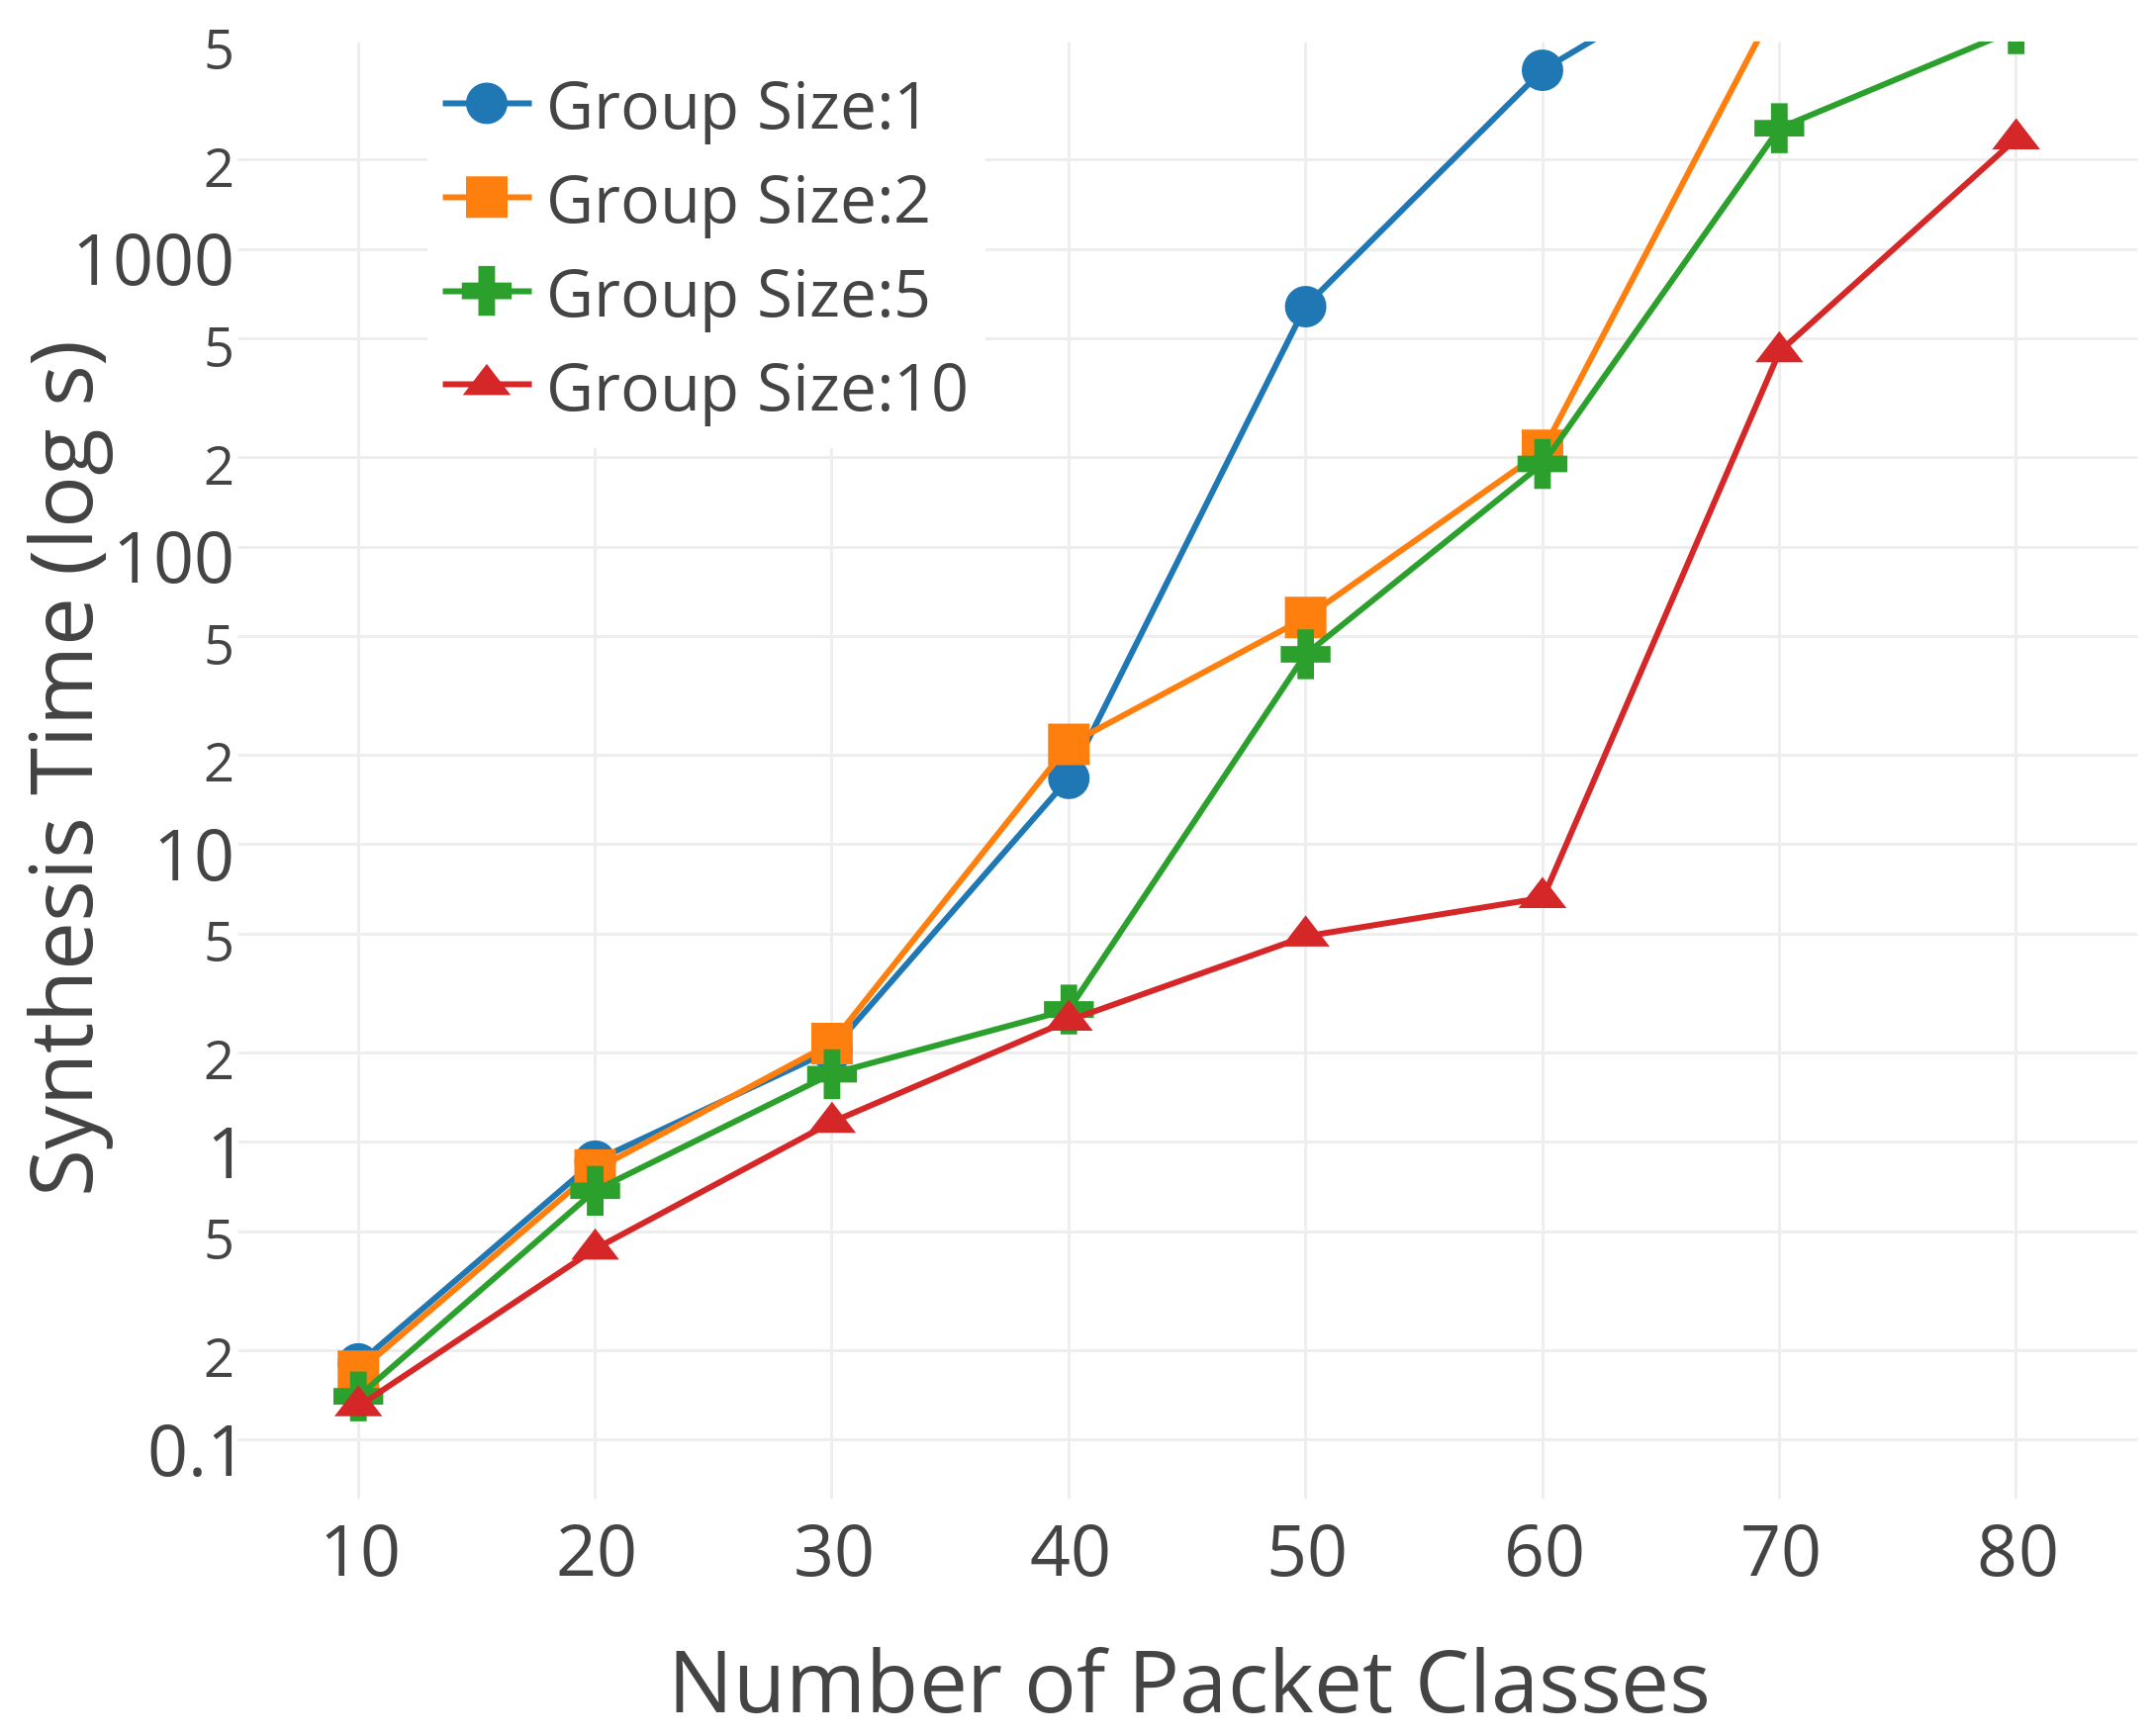
\includegraphics[width=0.66\columnwidth]{figures/no-tactic-isolation-plot.eps}}
	\subfloat[No Edge Tactic]{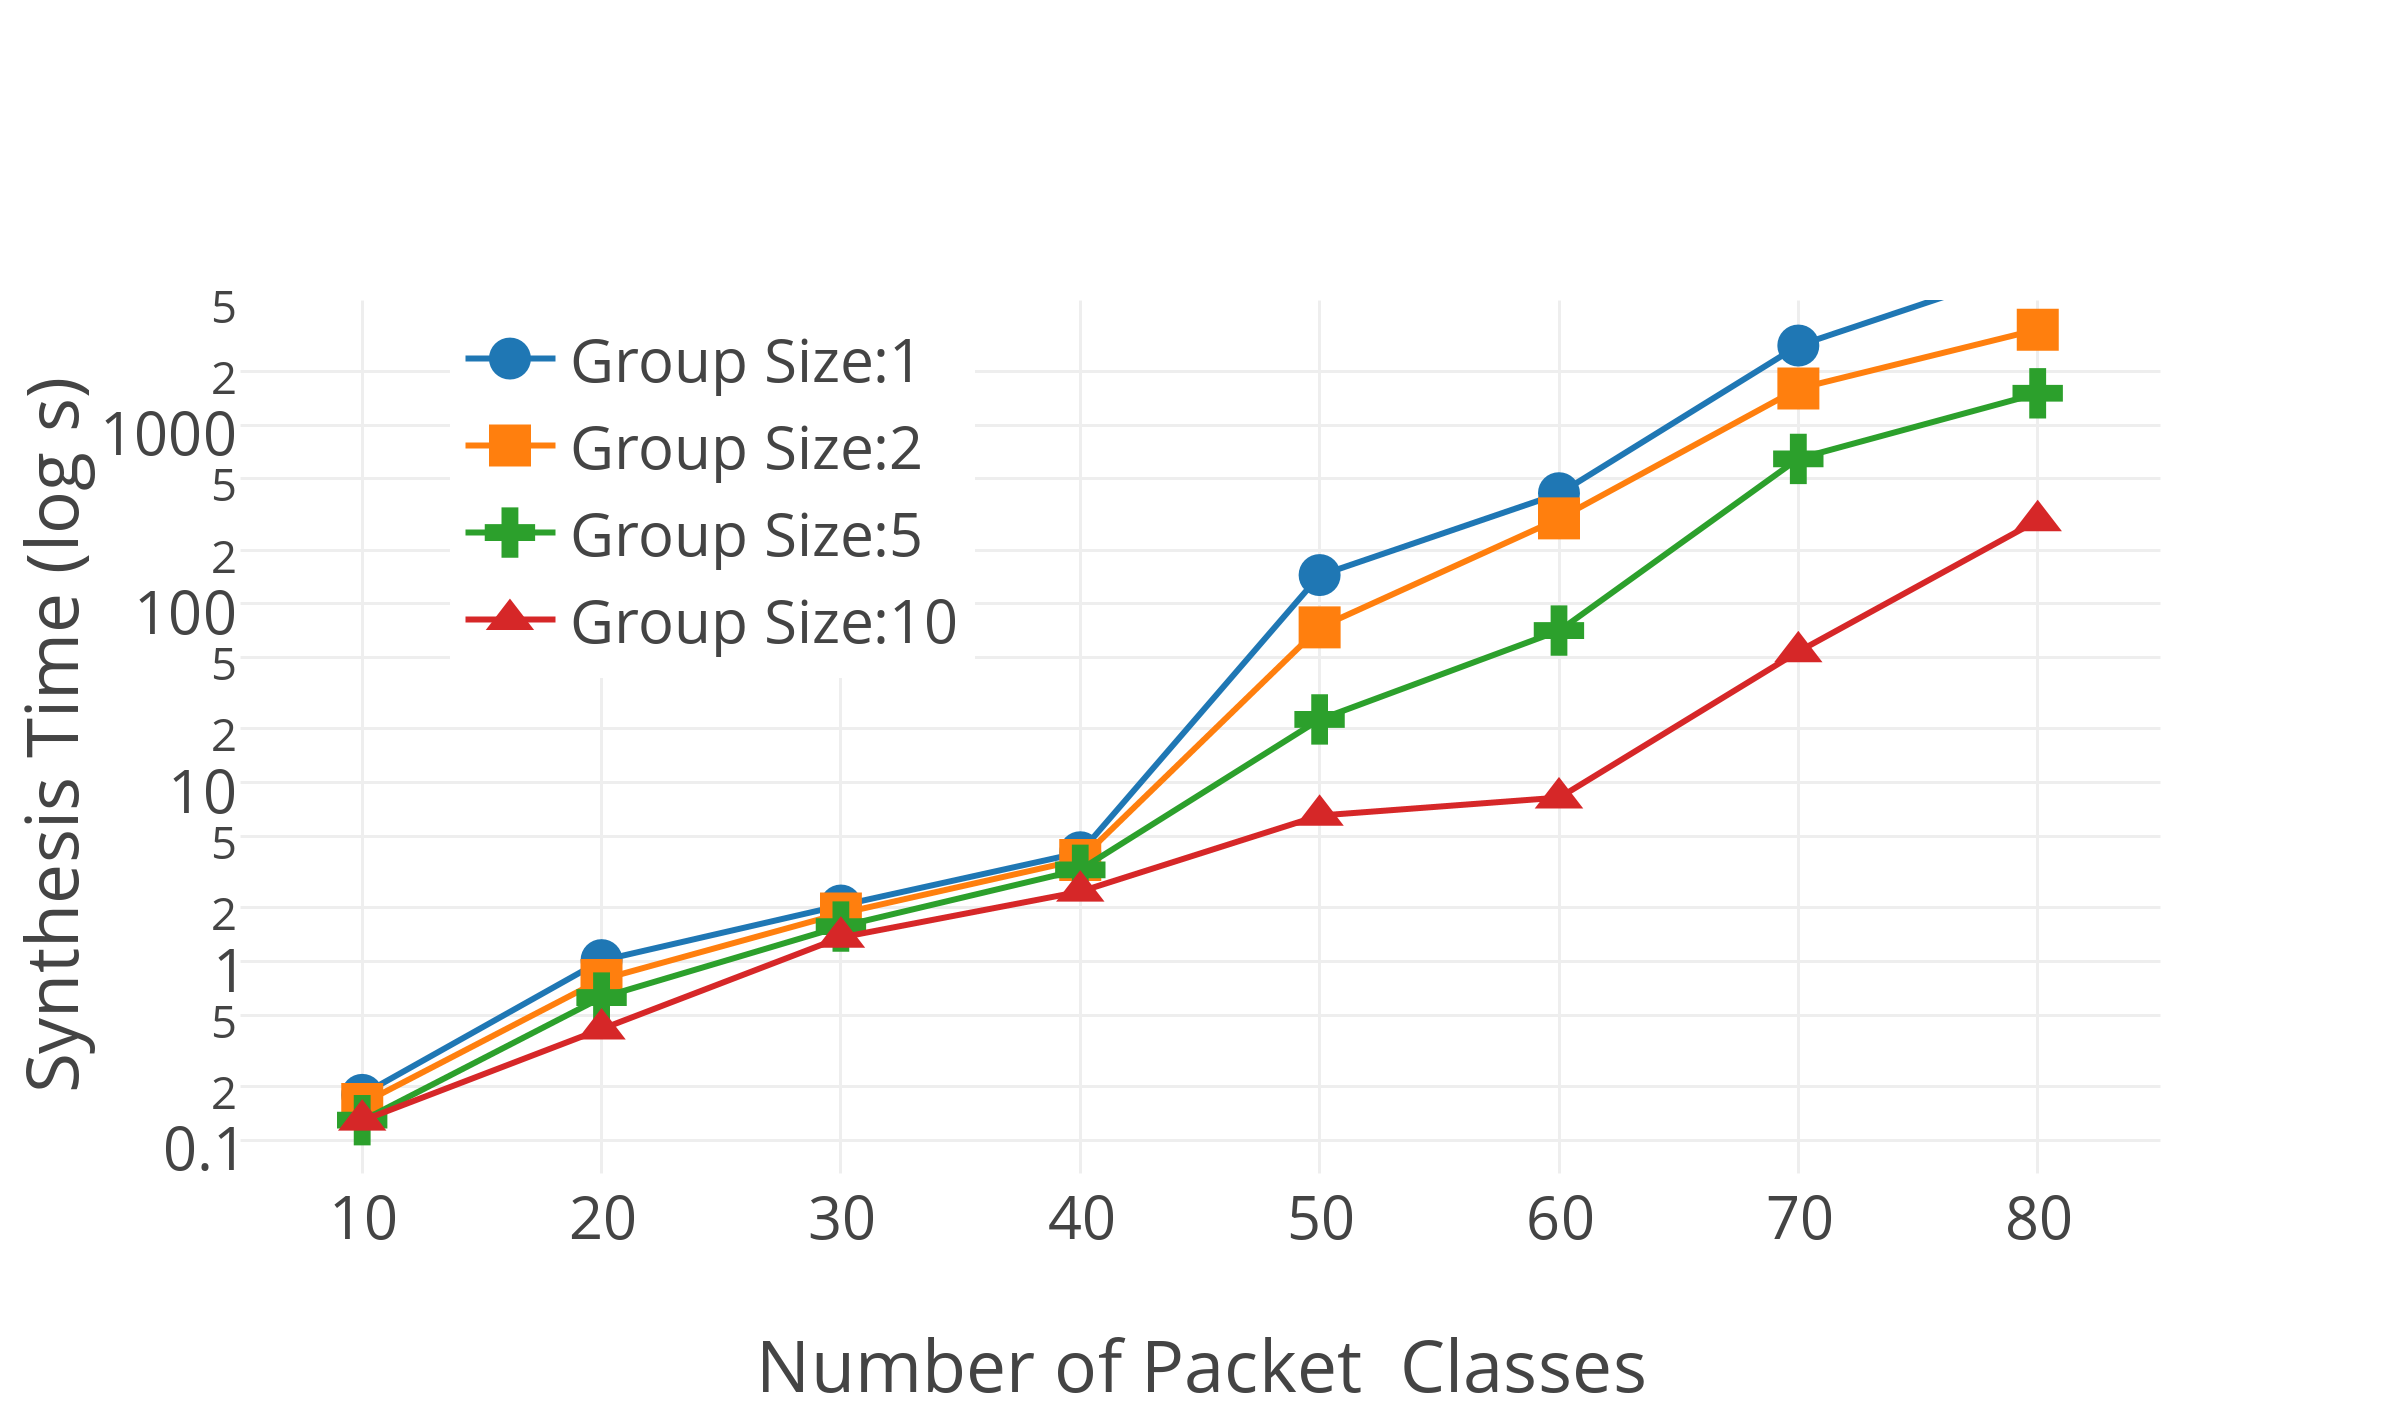
\includegraphics[width=0.66\columnwidth]{figures/no-edge-tactic-isolation-plot.eps}}
	\subfloat[Valley-free Routing Tactic]{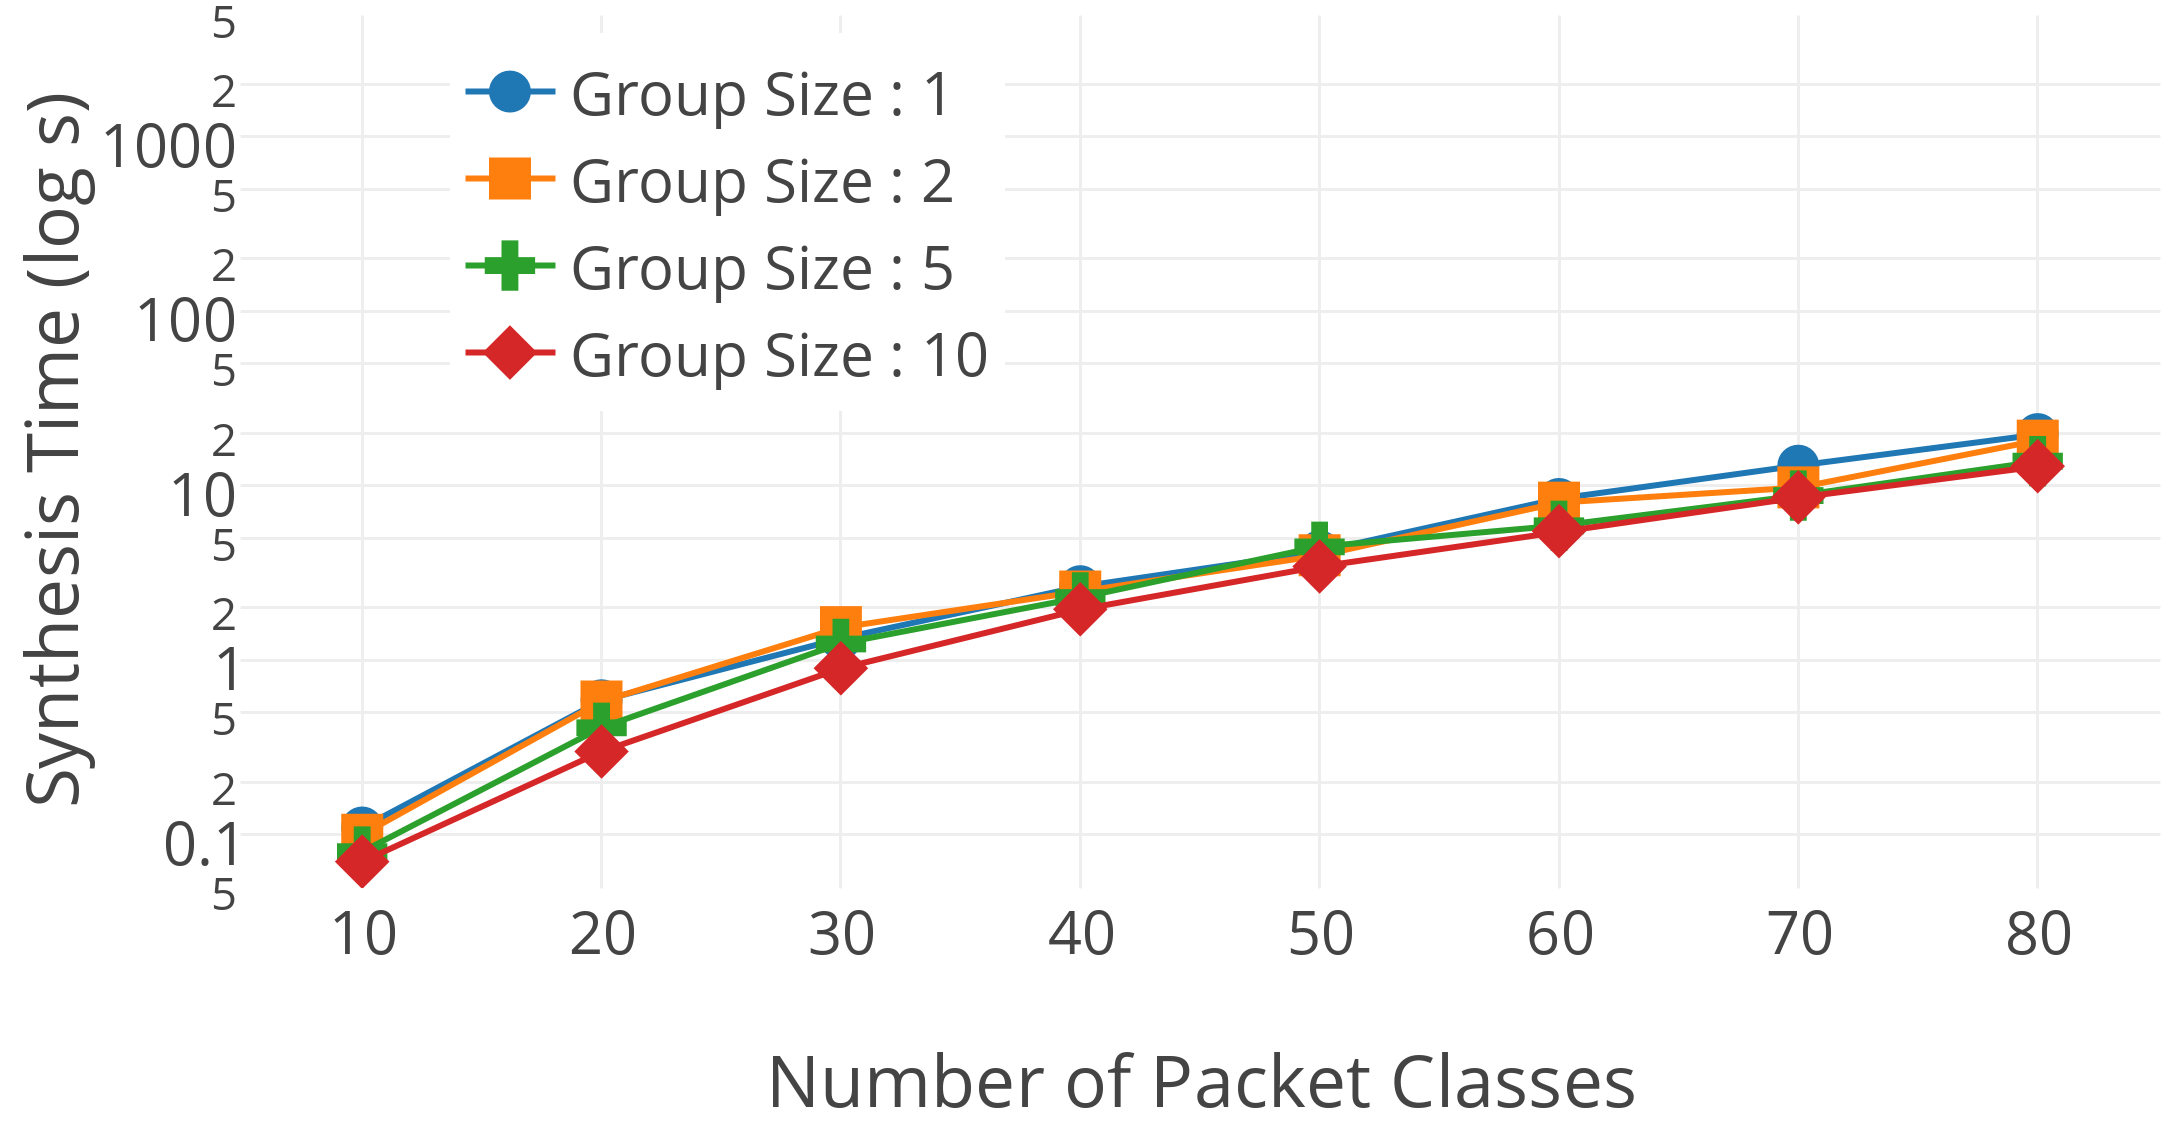
\includegraphics[width=0.66\columnwidth]{figures/eacae-isolation-plot.eps}}
	\caption{\label{fig:isolation}
		Total synthesis time (log scale) for isolation workloads over range of packet classes and different tenant-group sizes.}
\end{figure*}

\section{Evaluation} \label{sec:evaluation}

\noindent {\bf \Name Prototype:} We have implemented a full working
prototype of \Name in Python. We have implemented an interpreter for
the Genesis Programming Language using PLY~\cite{ply} and the synthesizer using 
the SMT solver Z3~\cite{z3} and its $\nu Z$ extension for MaxSMT and linear
 optimization~\cite{nuz3}; this outputs the
forwarding rules for the switches, which can be provided as input to a
SDN controller (for e.g., Floodlight~\cite{floodlight}) to install over the
network. \Name uses the Metis graph-partitioning library~\cite{metis}
to perform equi-sized partitioning 
used by divide-and-conquer synthesis.  The prototype contains 5K Python lines of code.  
We plan to make the code for \Name publicly available.

In this section, we evaluate \Name using
%\loris{really don't like the word realistic}
enterprise-scale multi-tenant data
center settings. 
Specifically, we ask:
\begin{compactitemize}

\item What is the performance of \Name's baseline synthesis
  algorithms? How does the performance vary with the size of the
  network, number of policies, and the nature of policies in use? (\secref{sec:baselineeval})
%  \loris{I usually write points like the following, but I'm not sure what's the standard
%  in systems conferences.
%We evaluate the performance using X with no optimization and consider
%different sizes of.... This experiment shows that...
%  }

\item How much do tactics help improve \Name's 
  performance? Which tactics offer the best improvement? (\secref{sec:tacticeval})

\item To what extent does the divide-and-conquer synthesis improve \Name's
  performance? When does it lead to degraded synthesis times? (\secref{sec:optimisticeval})

\item What is the performance of \name for traffic engineering and network repair
which makes use of SMT with linear optimization objectives, and MaxSMT? (\secref{sec:optimizationeval})

\end{compactitemize}
%\loris{if you say this here don't write it in the bullet points}
Our experiment settings have a few thousand servers, tens of switches,
and hierarchical fat-tree network topologies which reflect a private
datacenter. Our experiments are parameterized by: (a) total size of
the fat-tree network which we vary between 45 to 180 switches, (b) number of
tenants (1-80), and (c) number of packet classes in a tenant (1-10).

Our primary metric of interest is synthesis time, measured in
seconds. In measuring this, we focus on the time the Z3 solver takes
to solve the constraints\footnote{All experiments were conducted using a
	32-core Intel-Xeon 2.40GHz CPU machine and
	128GB of RAM.}. For evaluating the baseline performance, we impose a
synthetic limit on the path length $\mu$ to be $10$, which is more than adequate 
for a fat-tree topology with three levels. 

\subsection{Baseline Synthesis Performance} \label{sec:baselineeval} 
\noindent {\bf Multi-tenant Isolation}: To evaluate the baseline
performance of \Name without tactics, we model a multi-tenant 80 switch
 topology with tenant-isolation in
\Cref{fig:isolation}(a).  For each workload we have $n$ tenants with
group size $g$ which is the number of packet classes for each
tenant. The x-axis shows the total packet classes $n*g$.  Packet
classes of a tenant are not isolated (and they implement simple
reachability within the tenant), while packet classes of different
tenants are isolated. Thus, no two tenants share a link, and can never
affect each other's performance.  We randomly\footnote{ Smarter
  placement of tenants could speed-up synthesis as tenant endpoints
  would be located closer to each other. The placement algorithm can
  be used to develop specialized tactics.}  place endpoints for the
tenants' packet classes, ensuring that not more than 4 tenants share a
single edge switch.  Operators can aggregate a tenant's traffic from
one rack to another to a single reachability policy and establish
pathways for communication amongst the multiple machines in different
racks.

For a fixed group size, we can observe that, the total synthesis time
increases exponentially with increase in packet classes.  As we
decrease the group size, we can observe that synthesis time increases
greatly for the same number of packet classes.  In this case, the
number of tenants increases, making the problem more constrained due
to increased number of isolation policies.  Group size = 1 denotes the
extreme case where all flows are isolated w.r.t. one other.
 
While we evaluated a multi-tenant isolation setting, there are other
scenarios that translate to these workloads. Consider an example where
specific flows of tenants require QoS guarantees and these flows must
be isolated w.r.t all other flows. This translates to a two-tenant
isolation setting. Operators can provide weaker isolation such that
two flows must be isolated on only certain "special" links. 
This is an easier problem to tackle than isolation over all
links, and the performance of such scenarios would be better.

\noindent {\bf Effect of Topology Size}: To evaluate \Name across
increasing topology sizes for isolation workloads, we fix the
tenant-group size to 5, and for each topology, we maintain the ratio
of packet classes to number of edge-aggregate links to 0.25.  We
choose this metric because if we kept the number of classes constant,
as topology sizes increases, it is easier to find isolated
paths. Thus, by keeping the number of packet classes proportional to
size of the topology, we maintain the relative difficulty of the
workload across topologies.  We show the average synthesis time per
class with increasing topology sizes in
\Cref{fig:tactic-topo}.  We are able to synthesize forwarding rules
for 12 tenants with tenant-group size 5 in a 125 switch topology in 124
seconds (avg. 2 seconds per traffic class).
 %Some comment I dont understand.
We can also observe that average time per flow increases exponentially
with larger topologies, thus the synthesis problem is also exponential
in number of switches.
  
  
 \noindent{\bf Isolation with Link Capacity Policies}: 
 \Cref{fig:link-capacity}(orange trace) shows the average synthesis time per flow for the same setting, but
 additionally, there are 10 low-bandwidth links in the network for which the operator
 specifies policies to capacity usage (all packet classes have uniform capacity). 
Since we use LIA for link capacity constraints, we see an 
increase in average time for synthesis 
when compared to pure isolation which is completely 
encoded using SAT. 

\noindent {\bf Waypoint Policies}: To evaluate \Name's performance for
ordered sets of waypoints, we fix the number of waypoints (range:1-5)
and generate 100 waypoint policies with different size and permutation
of the ordered waypoint sets for a 80 switch topology. Each
policy has edge switches as endpoints and randomly picked core or
aggregate switches for waypoints. The synthetic limit $\mu$ on the
path length is increased to 15 and no tactics are used (
difficult to devise a tactic for the path satisfying a waypoint policy). The
average synthesis time for a waypoint policy is reported in
\Cref{tab:waypointeval}.  We observe that synthesis time increases
exponentially with total number of waypoints in a packet class's
policy, owing to the complexity of the problem.  \Name can synthesize
rules for a path with 3 total waypoints in less than a second on
average. These waypoint policies were either completely ordered or
unordered or waypoint sets of sizes 1 and 2.
%\aditya{I don't follow this last sentence}

\begin{table}
\begin{footnotesize}
	\begin{center}
		\begin{tabular}{P{6em} | P{7em}} 
			Number of Waypoints & Avg. Synthesis time per Class (s) \\ [0.5ex] 
			\hline
			1 & 0.0347\\ [0.5ex] 
			\hline
			2 & 0.1384\\ [0.5ex] 
			\hline
			3 & 0.9834\\ [0.5ex] 
			\hline
			4 & 15.41\\ [0.5ex] 
			\hline
			5 & 32.93\\ [0.5ex] 
		\end{tabular}
	\end{center}
	\compactcaption{Average synthesis time per class for waypoint policies with increasing number of waypoints. } \label{tab:waypointeval} 
\end{footnotesize}
\end{table}
 % Write about waypoints
 \subsection{Tactic Reductions} \label{sec:tacticeval}
 Using the baseline synthesis approach can result in high synthesis
 times due to the large solution space of forwarding plane configurations. We 
 demonstrate the improvements from using tactics for different tenants and group sizes on a 
 80 switch topology.
 
 \noindent {\bf No Edge Tactic}: \Cref{fig:isolation}(b) shows the synthesis time for isolation workloads using the no edge tactic 
 ($\neg(e .^* e .^* e)$). We achieve a best-case speedup of 9.5$\times$ over baseline synthesis with this tactic. 
 Using this tactic, \Name can synthesize forwarding rules for 12 tenants with group size 5 in under 200
 seconds.
  
\noindent {\bf Valley-free Routing Tactic}:  
For the same isolation workloads as above, we use the tactic $\neg (e .^5 .^* e)$ $\wedge \neg (e .^* e .^* e)$
 which ensures {\em valley-free routing}, that is paths are of the form $eacae$. 
 The results are shown in \Cref{fig:isolation}(c). 
 Using this tactic, \Name synthesizes forwarding rules for each workload in under 20 seconds 
 and can achieve a best-case reduction of 400$\times$ compared to synthesis without tactics. 
 
 \begin{figure}[h]
 	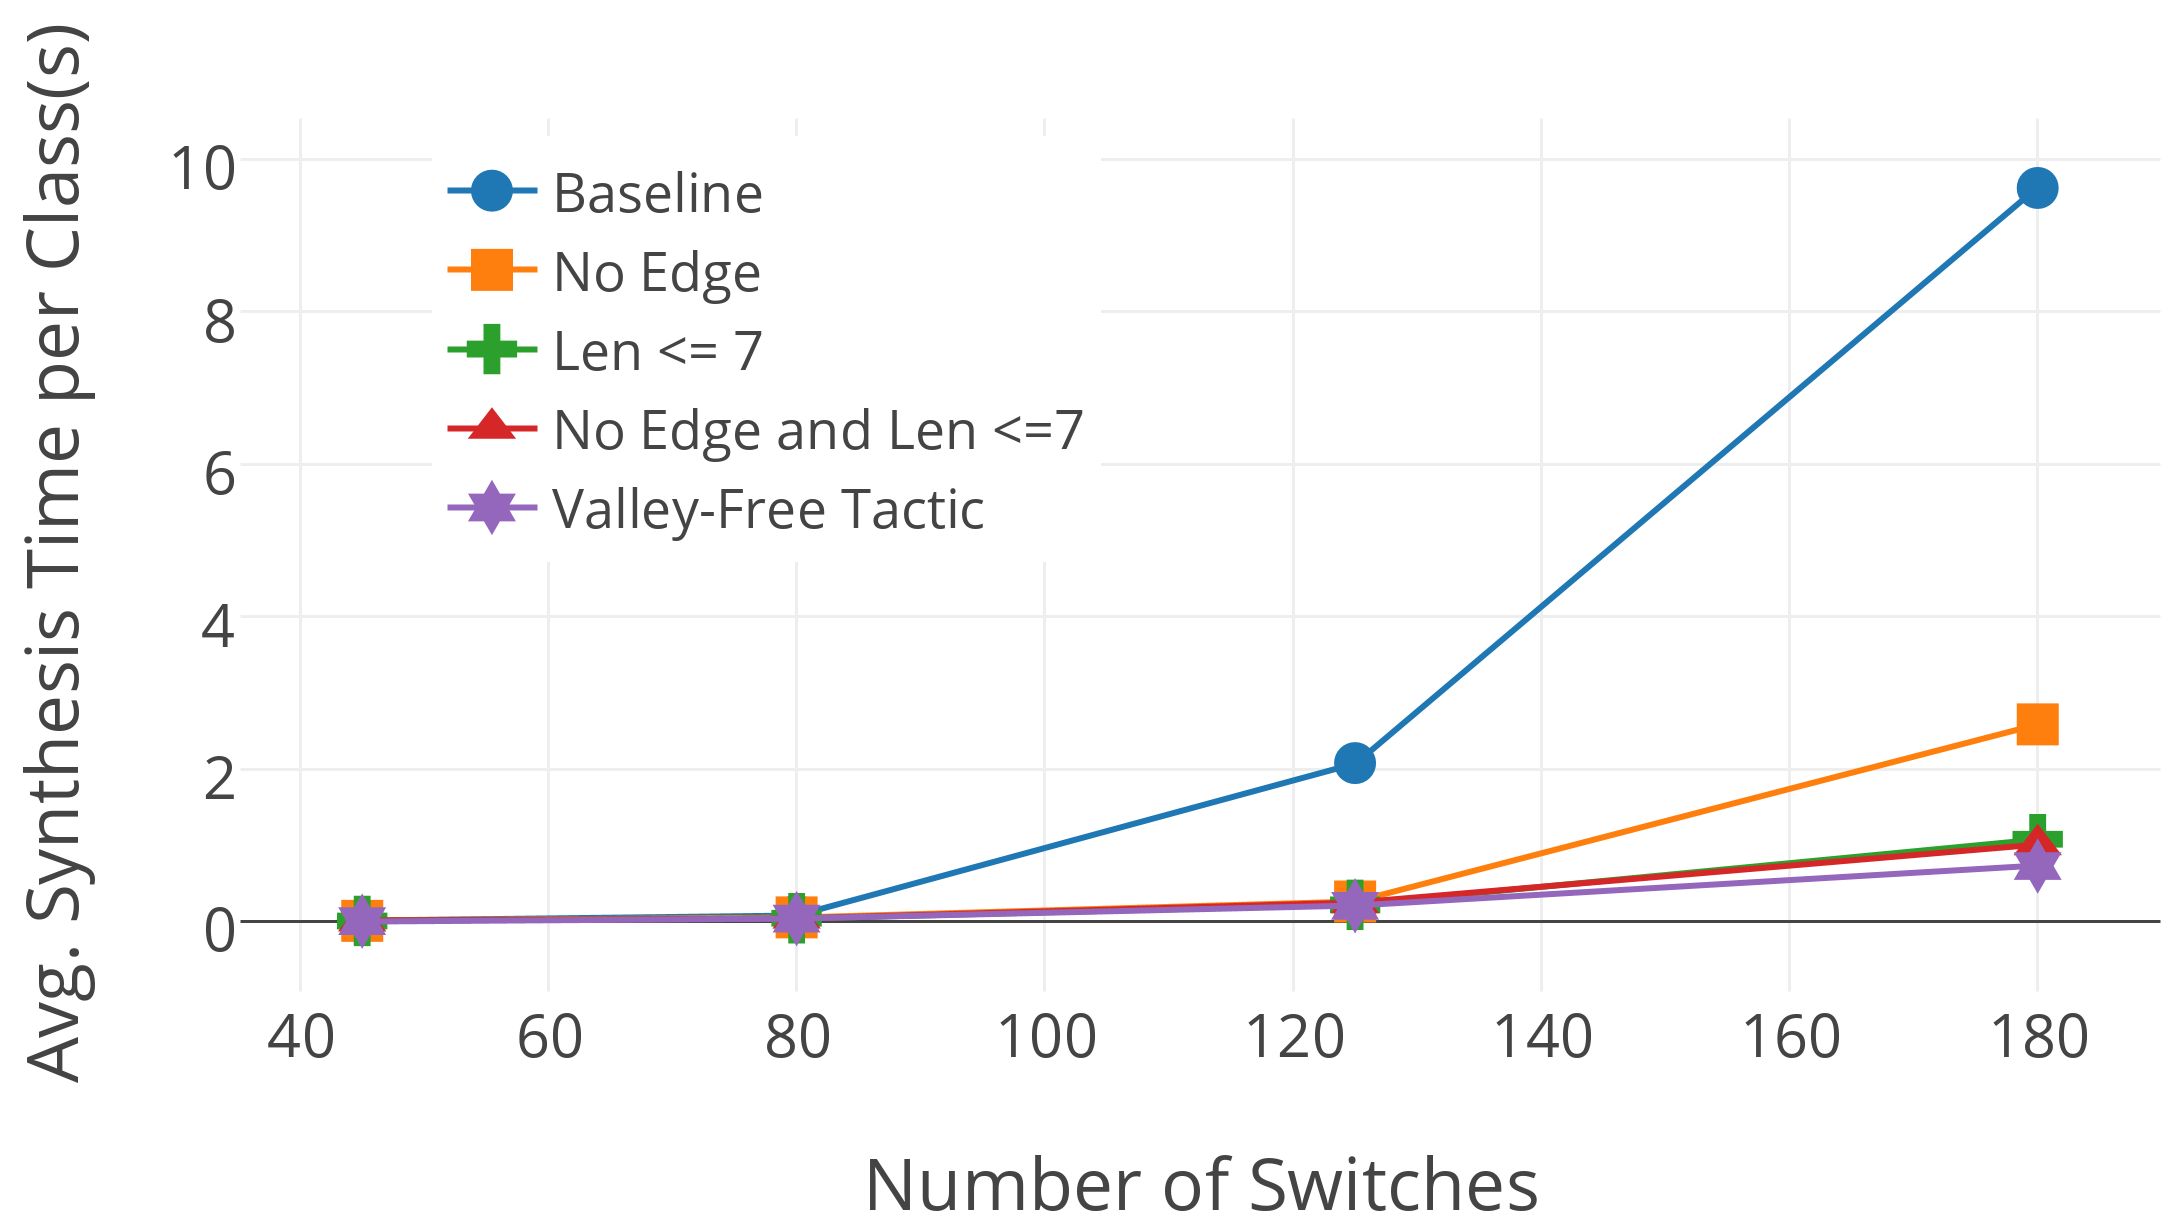
\includegraphics[width=\columnwidth]{figures/tactic-topo.eps}
 	\caption{Average synthesis time per packet class versus topology size for isolation workloads 
 		w/o different tactics with the ratio of packet classes to number of edge-aggregate links 0.25.}
 	\label{fig:tactic-topo}
 \end{figure}
 
\noindent {\bf Effect of Topology Size}: 
In \Cref{fig:tactic-topo},
 we evaluate the performance of different tactics for different topology sizes. There is a
 significant reduction of synthesis time for each tactic when compared to the baseline synthesis.
 The performance of each tactic is directly related to the reduction of the solution space: a more
 restrictive tactic has lower synthesis times. 
  Using the no edge tactic
 and path length $\leq 7$ tactic, \Name synthesizes forwarding rules for 20 tenants of group-size 5 in 100 seconds in a 180 switch
 topology (9$\times$ speedup over synthesis without tactics).
  
 \noindent{\bf Isolation with Link Capacity Policies}: A similar setup
 with additional link capacity constraints for 10 links is evaluated
 using the no edge tactic, and we get a best-case 14$\times$
 improvement over baseline synthesis. This demonstrates the usefulness
 of tactics for integrating different kinds of policies like isolation
 and link capacities.  Tactics can provide a considerable improvement
 over the baseline performance as illustrated by these experiments,
 and demonstrate the viability of synthesis approach of \Name to
 real-world networks.
 
\begin{figure}[h]
	\centering
	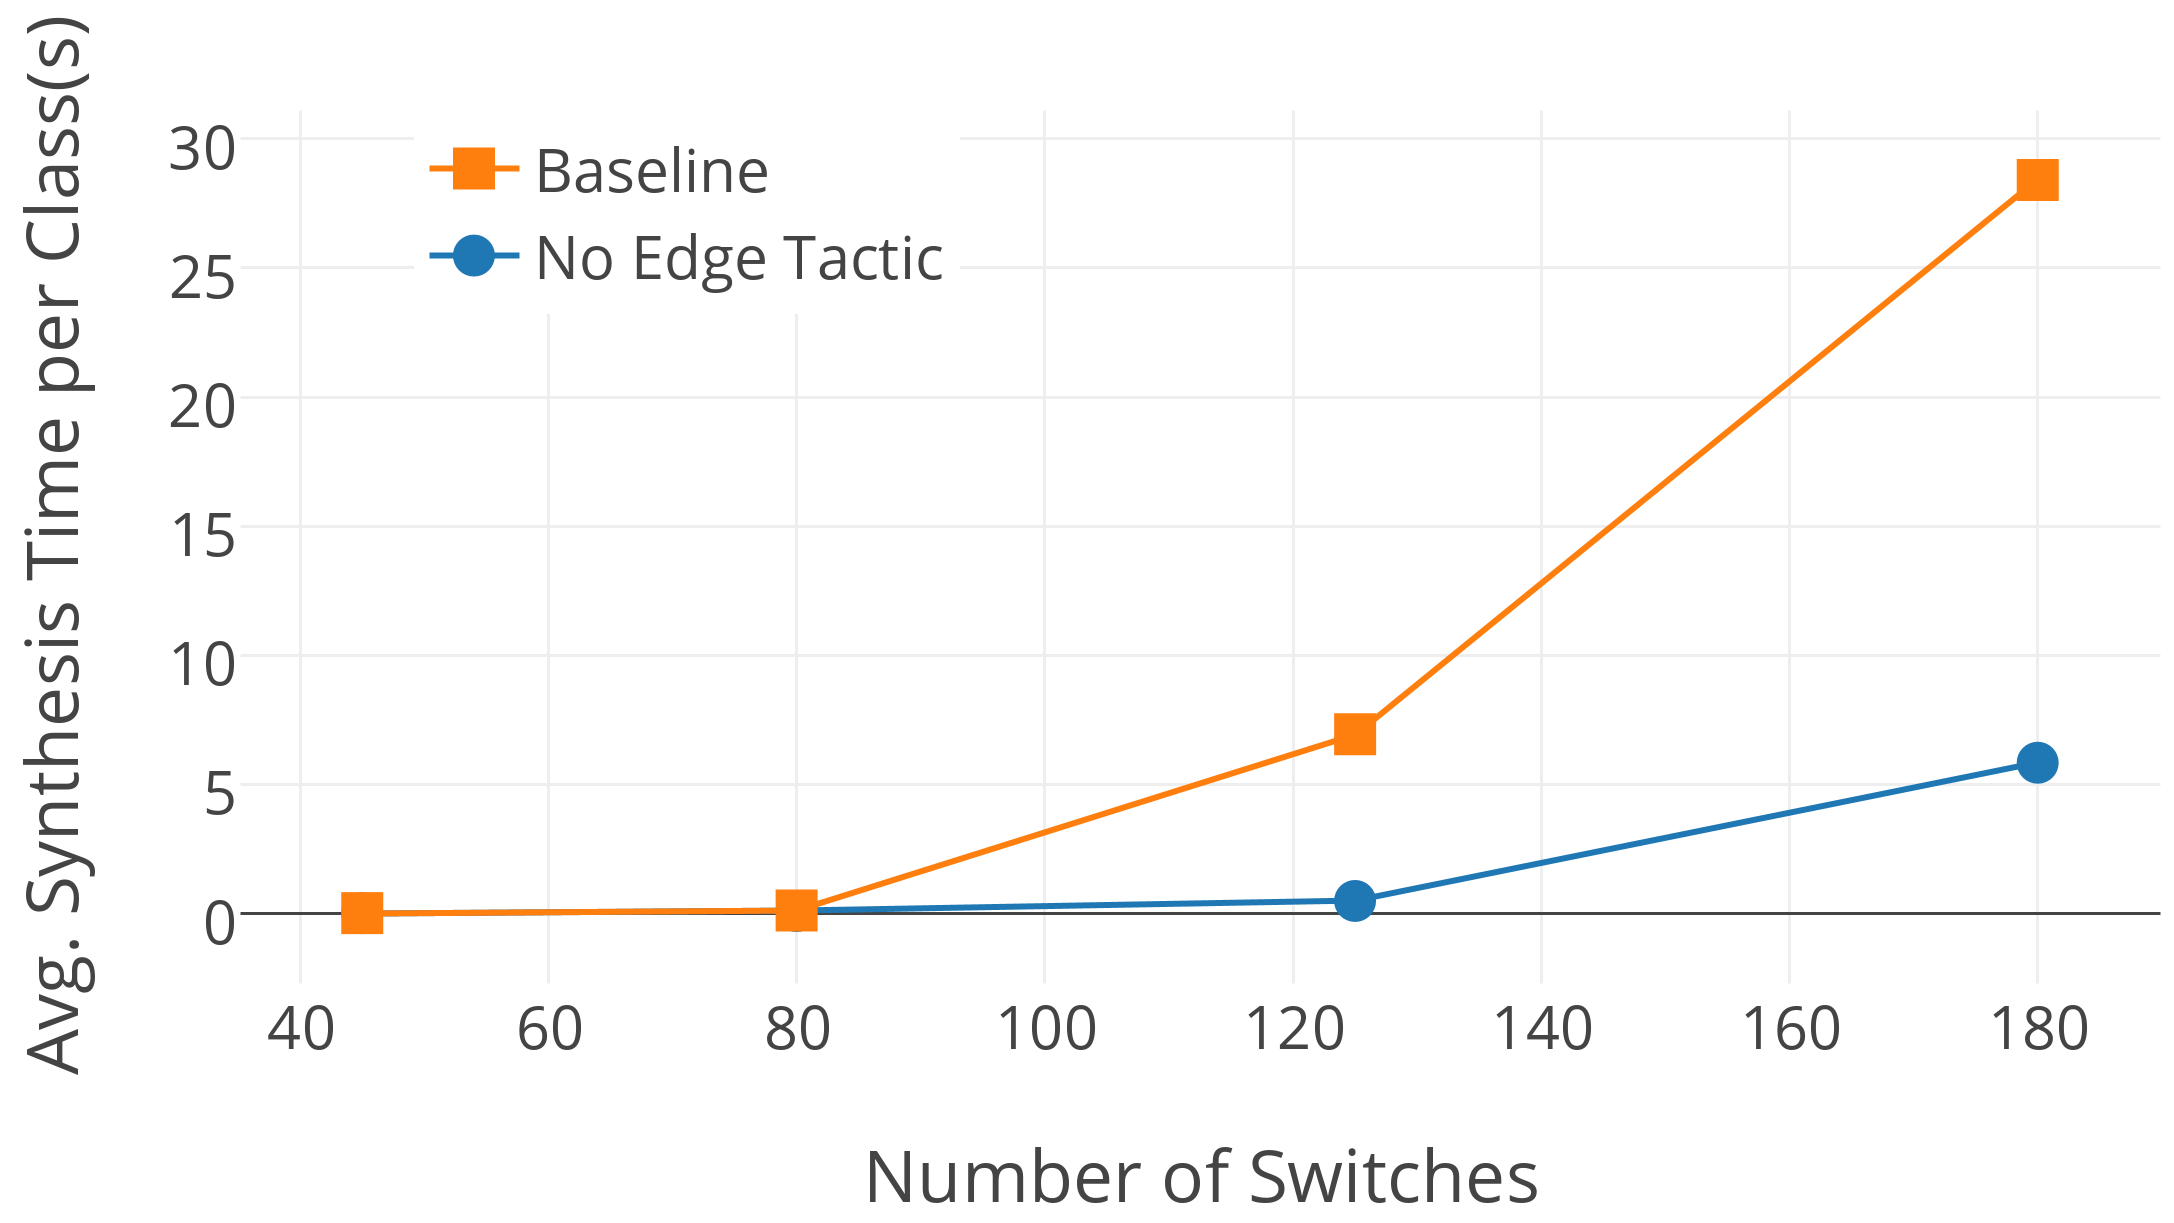
\includegraphics[width=0.75\columnwidth]{figures/link-capacity-plot.eps}
	\caption{Average synthesis time per packet class versus topology size for isolation workloads 
		with the ratio of packet classes to number of edge-aggregate links 0.25 and 10 low bandwidth links in the topology 
		have capacity policies.}
	\label{fig:link-capacity}
\end{figure}

\begin{figure}
	\centering
	\includegraphics[width=0.75\columnwidth]{figures/dcsyn-cdf.eps}
	\caption{CDF for speedup achieved by divide-and-conquer synthesis.}
	\label{fig:dcsyn-cdf}
\end{figure}
\subsection{Divide-and-Conquer (DC) Synthesis Performance} \label{sec:optimisticeval} 
To evaluate the heuristic
divide-and-conquersynthesis procedure, we perform 100 runs of non-heuristic
synthesis and divde-and-conquer synthesis (with the no edge tactic in both cases) on
isolation workloads with varying number of tenants and different group
sizes we used in the \Cref{fig:isolation} experiment. We compute the
speedup (time of non-DC synthesis/time of DC synthesis) and plot its cumulative
frequency distribution in \Cref{fig:dcsyn-cdf} to quantify the benefits
of optimistic synthesis. For more than 80\% of the workloads,
divide-and-conquer offers a better or comparable performance to non-optimistic
synthesis, achieving a speedup of 2$\times$ for nearly 40\% of the
workloads. For 20\% of the workloads, divide-and-conquer performs worse than
the non-heuristic approach, especially for workloads with tenant
group size 1.  This arises due to greater recovery attempts which
results in increased time. We can leverage parallelism by running 
both instances of synthesis, thus giving the best performance, with
or without the divide-and-conquer approach.

\begin{table}
	\begin{footnotesize}
		\begin{center}
			\begin{tabular}{P{7em} | P{13em} | P{4em}} 
				Workload Type & Description & Synthesis Time (s) \\ [0.5ex] 
				\hline 
				\multirow{2}{*}{minimize-avg-te}& 100 packet classes & 425 \\ [0.5ex]
				 & 200 packet classes & 2002 \\ [0.5ex]
				\hline
					\multirow{2}{*}{minimize-max-te} & 25 packet classes & 522 \\ [0.5ex]
					& 50 packet classes & 4192 \\ [0.5ex]
				\hline
				Network repair & 8 tenants, group size 10, tenant-isolation, one switch failure & 219 \\ [0.5ex]
			\end{tabular}
		\end{center}
		\compactcaption{Synthesis times for workloads on a 80-node fat-tree topology with different optimization objectives.} \label{tab:optimizeval} 
	\end{footnotesize}
\end{table}
\subsection{Synthesis with Optimizations} \label{sec:optimizationeval}
\Cref{tab:optimizeval} shows the synthesis time for workloads on a 80-node fat-tree topology
with different optimization objectives like traffic engineering and network repair. \name can
 do traffic engineering with minimizing average utilization for 200 packet classes in ~2000 seconds. However,
 for minimizing the maximum link utilization, \name can only synthesize 50 packet classes in ~4000 seconds. For both
 objectives, the synthesis time increases exponentially to increasing number of packet classes. SMT with
 optimization objectives is an emerging field of research, and we envision that solvers in the future will become fast
 to handle larger workloads. 
 
 To evaluate the performance of network repair using MaxSMT, we consider such a 
 setting. There are 8 tenants, each with 10 packet classes (total classes=80), and tenant
 flows are isolated from one another. Now, we disable the switch with the largest number 
 of rules, and try to find a new configuration from the old one with maximum number of switches
unaffected, and the new configuration satisfies the original tenant isolation policies, and we can
synthesize the minimal repair in ~200 seconds. 

\minisection{Summary} The key points of our evaluation are:
\begin{compactitemize}
\item For a representative tenant-group size of 10 in a 80 switch
  fat-tree, the baseline synthesis performance for synthesizing the
  forwarding rules for 1 to 8 tenants with complete tenant-isolation
  is in 0.1-2000s;
      \item Tactics provide considerable improvement over the
        baseline, making \Name practical.  We can synthesize the above
        workloads in 0.1-300s using the no edge tactic,
        and under 12s using the valley-free routing tactic;
      \item \Name can effectively tackle real-world scenarios using
        optimistic synthesis, which provides a 2.0$\times$ speed-up
        over non-optimistic synthesis in 40\% of the workloads, in
        addition to the tactic improvements;
        \item Adding optimization objectives with SMT for TE and using
        MaxSMT for network repair is more expensive than synthesis without
        objectives.
\end{compactitemize}


%\begin{figure*}
%	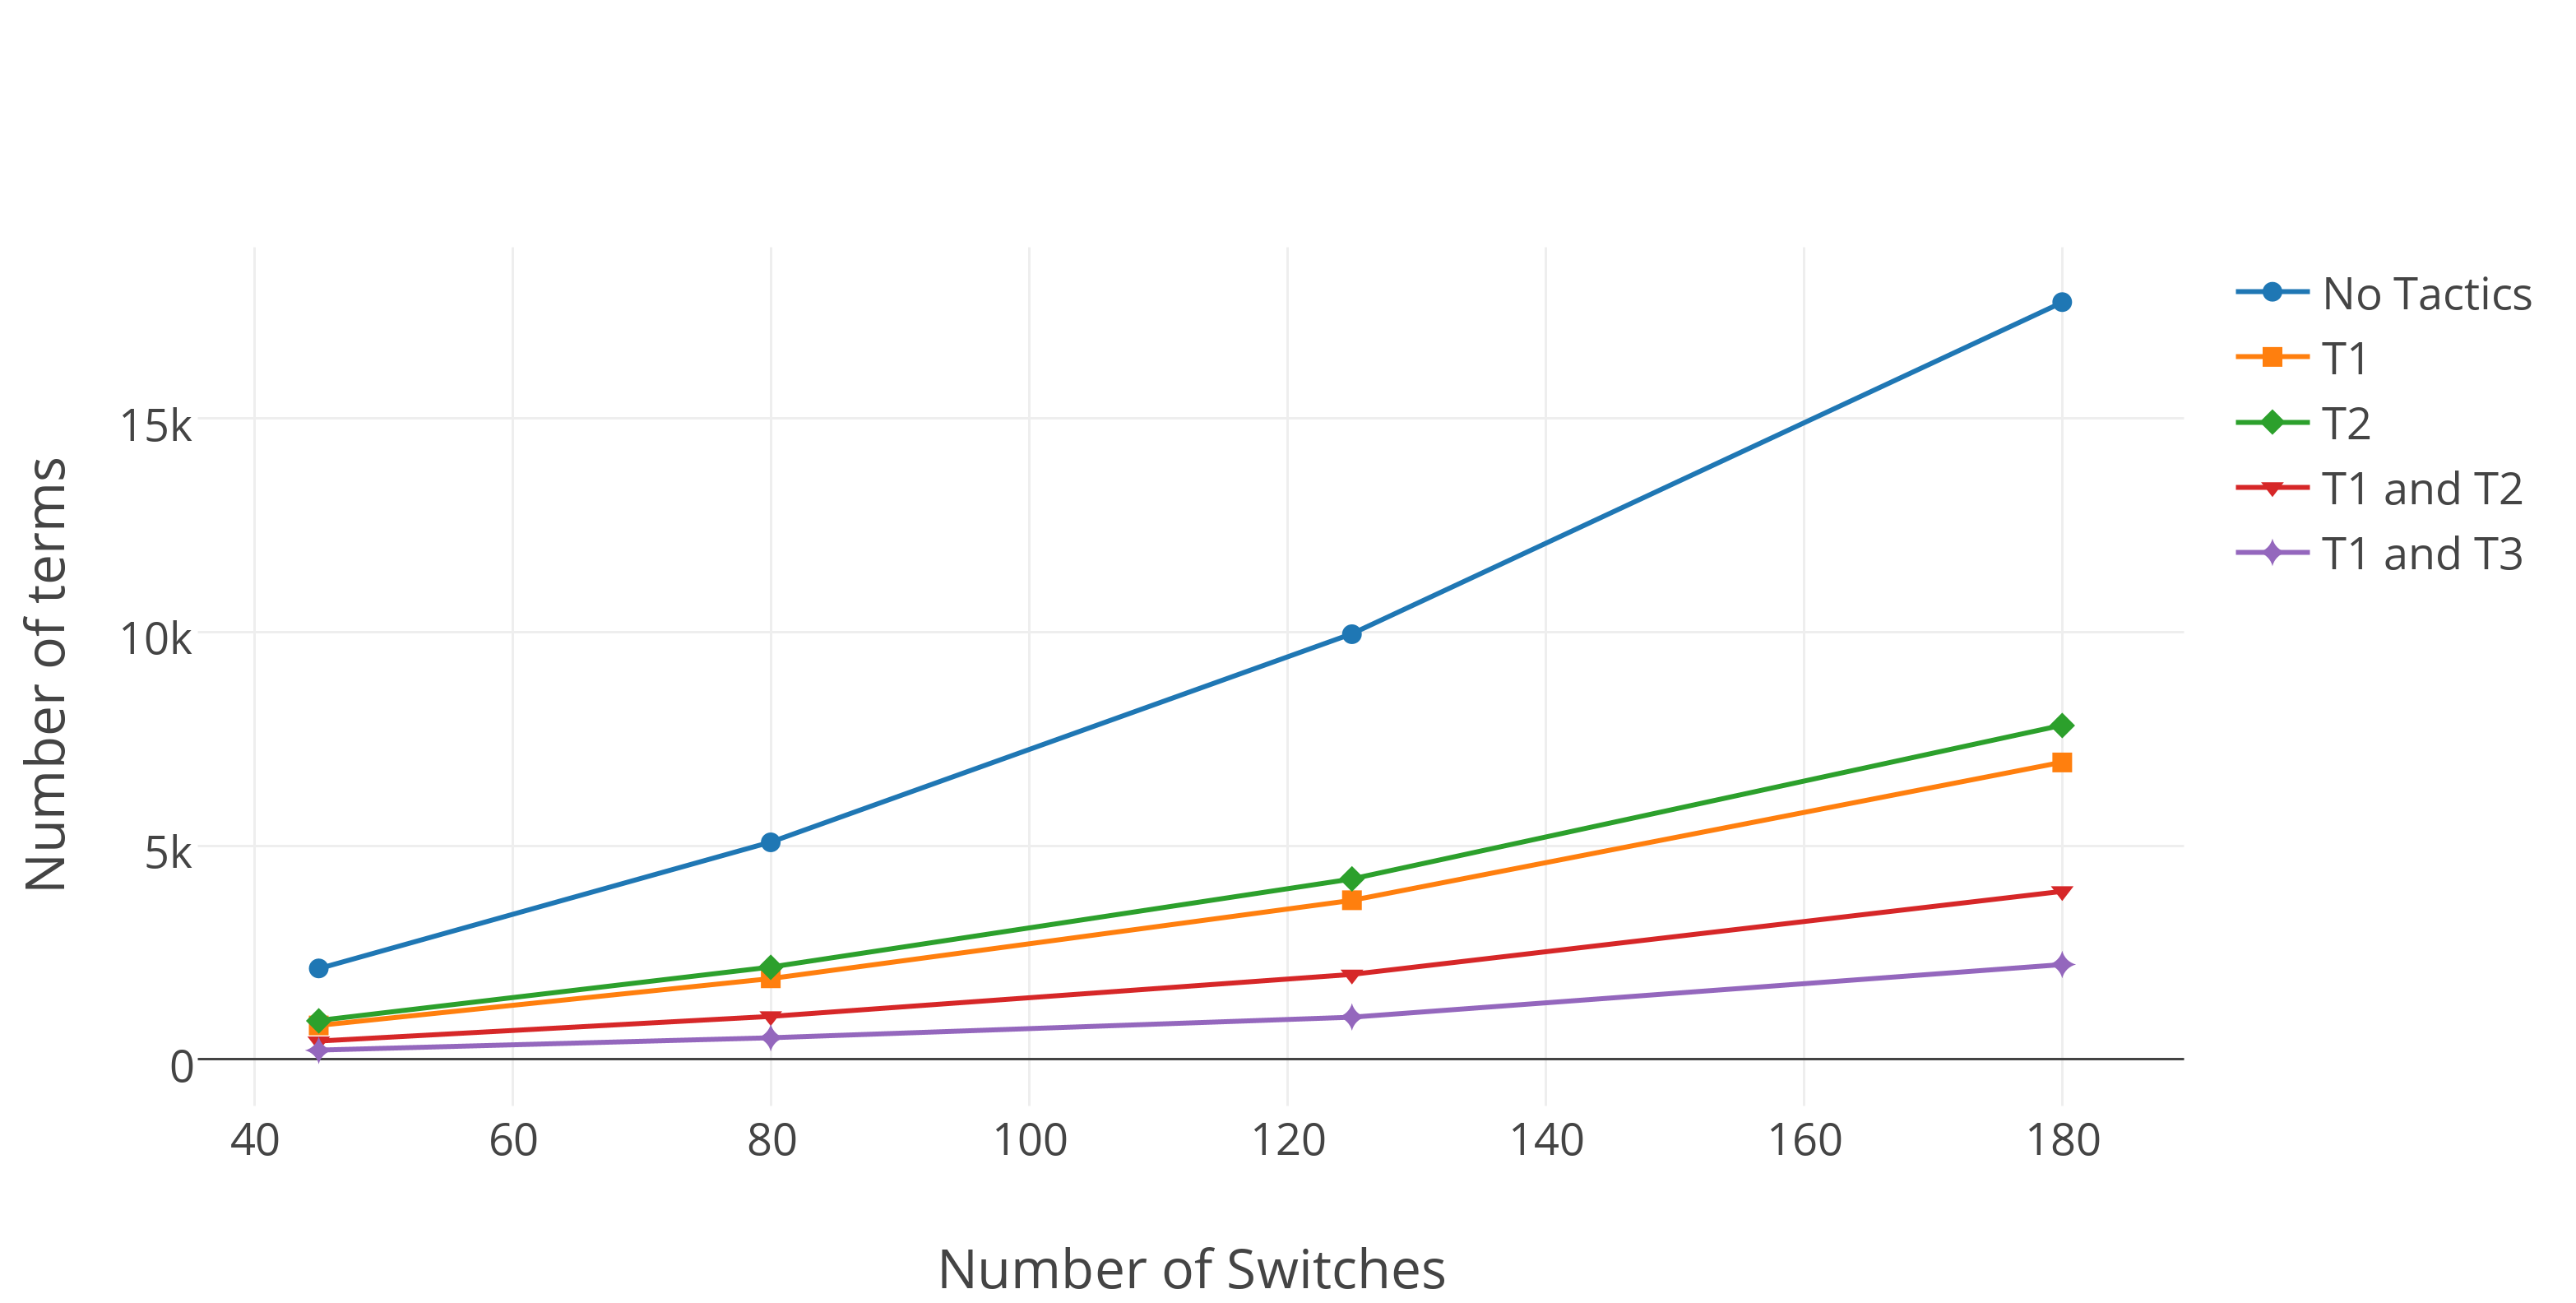
\includegraphics[height=7.5cm]{figures/tactic-reduction.png}
%	\caption{Graph used to show the reduction of terms using different tactics w.r.t the total number of terms}
%	\label{fig:tactic-reduction}
%\end{figure*}
%
%\begin{figure}
%	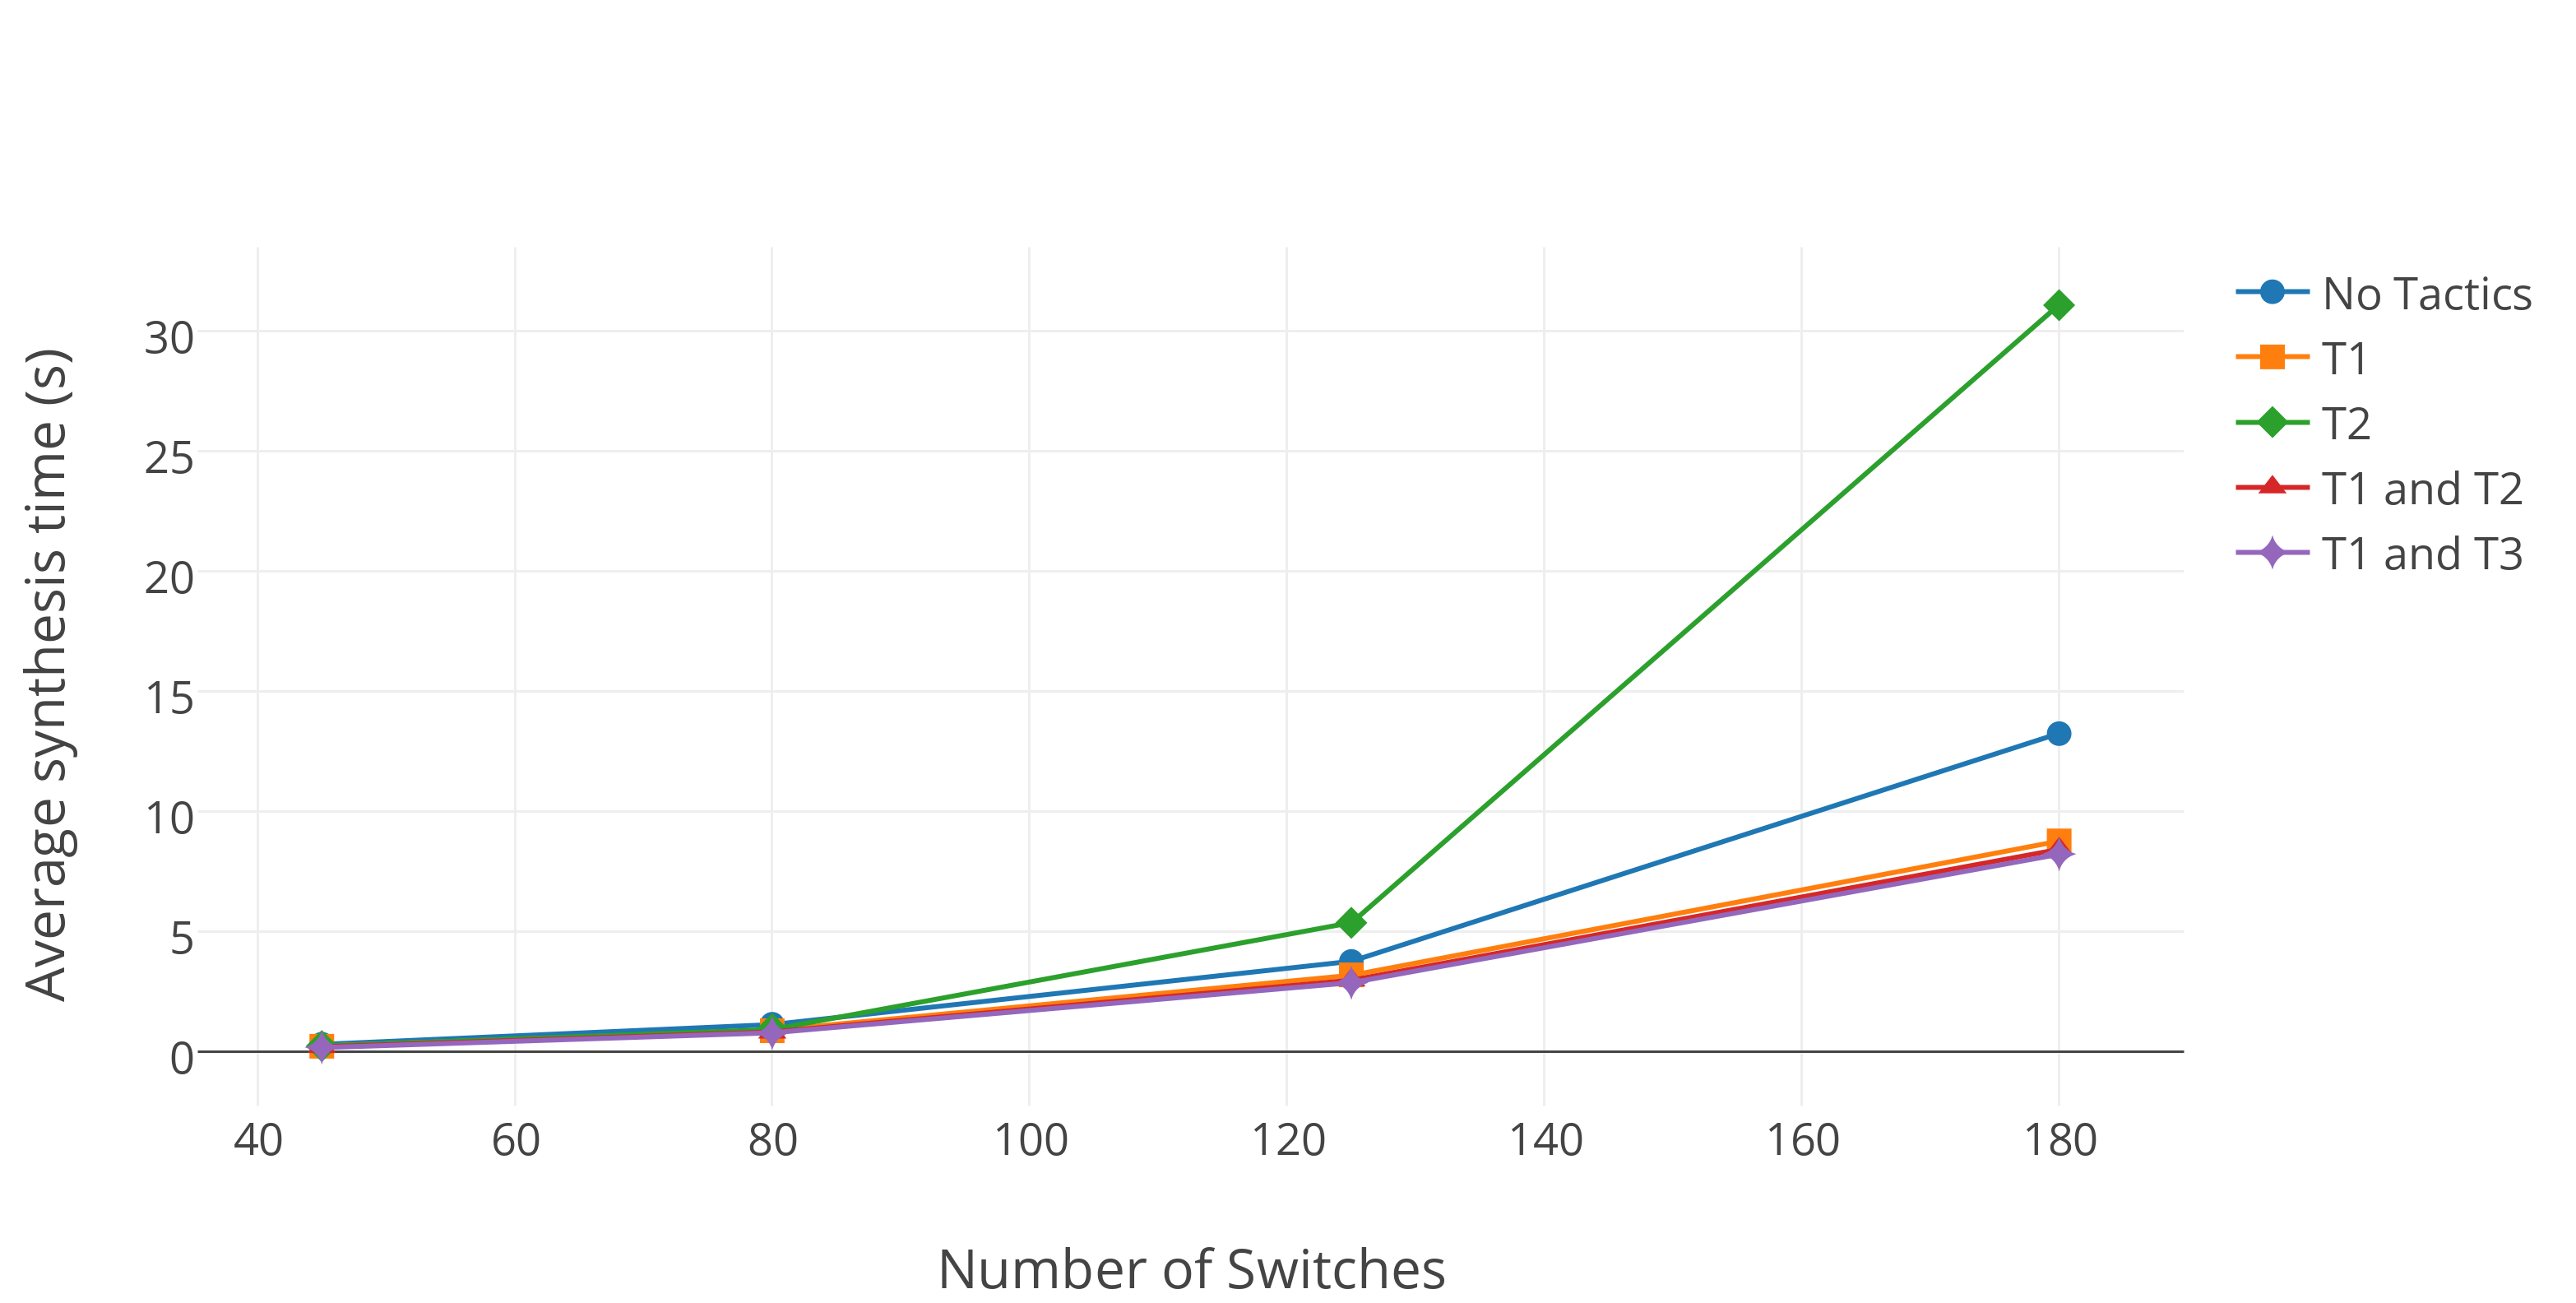
\includegraphics[width=\columnwidth]{figures/isolation-tactics.png}
%	\caption{Graph used to application of tactics for a isolation workload (percentage isolation w.r.t topology 25\%) and different topology sizes. An interesting observation in the graph is that tactics need not always help in reduction of constraints (One of the tactics, not  a very natural one) leads to more time to synthesis without tactics.}
%	\label{fig:isolation-tactics}
%\end{figure}
%
%\subsection{Optimistic Synthesis}

%\begin{figure}
%	\centering
%	\subfloat[Optimistic]{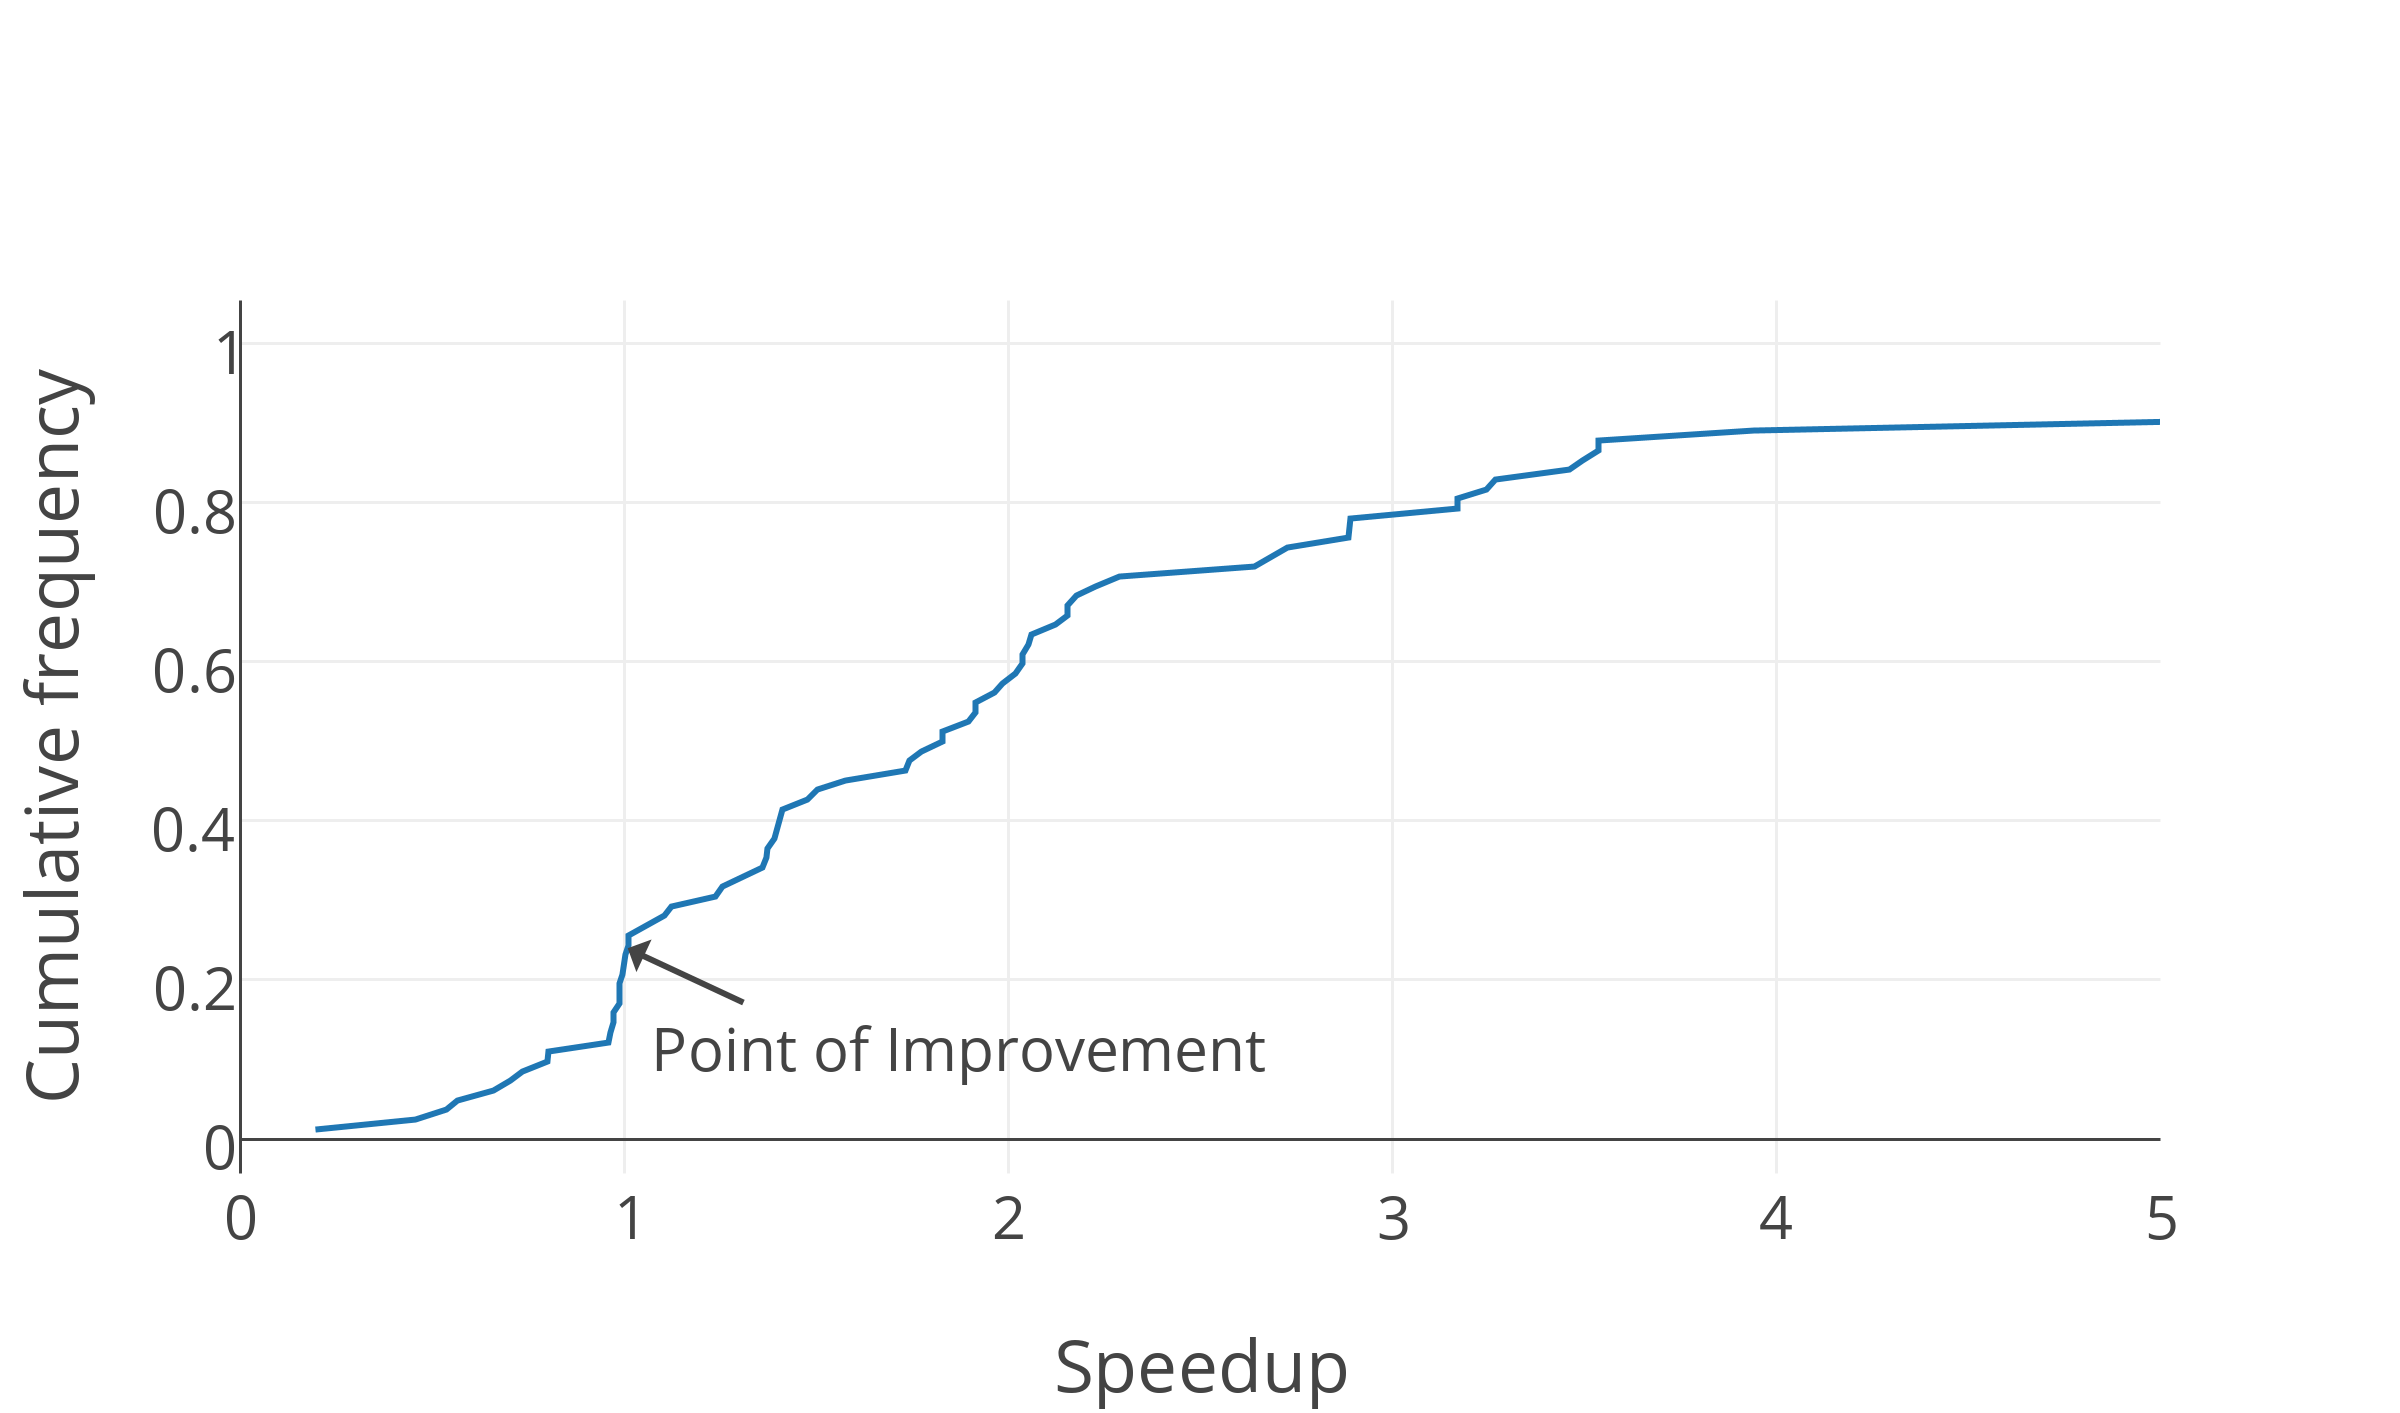
\includegraphics[width=0.5\columnwidth]{figures/opt-cdf.eps}}
%	\subfloat[Incremental]{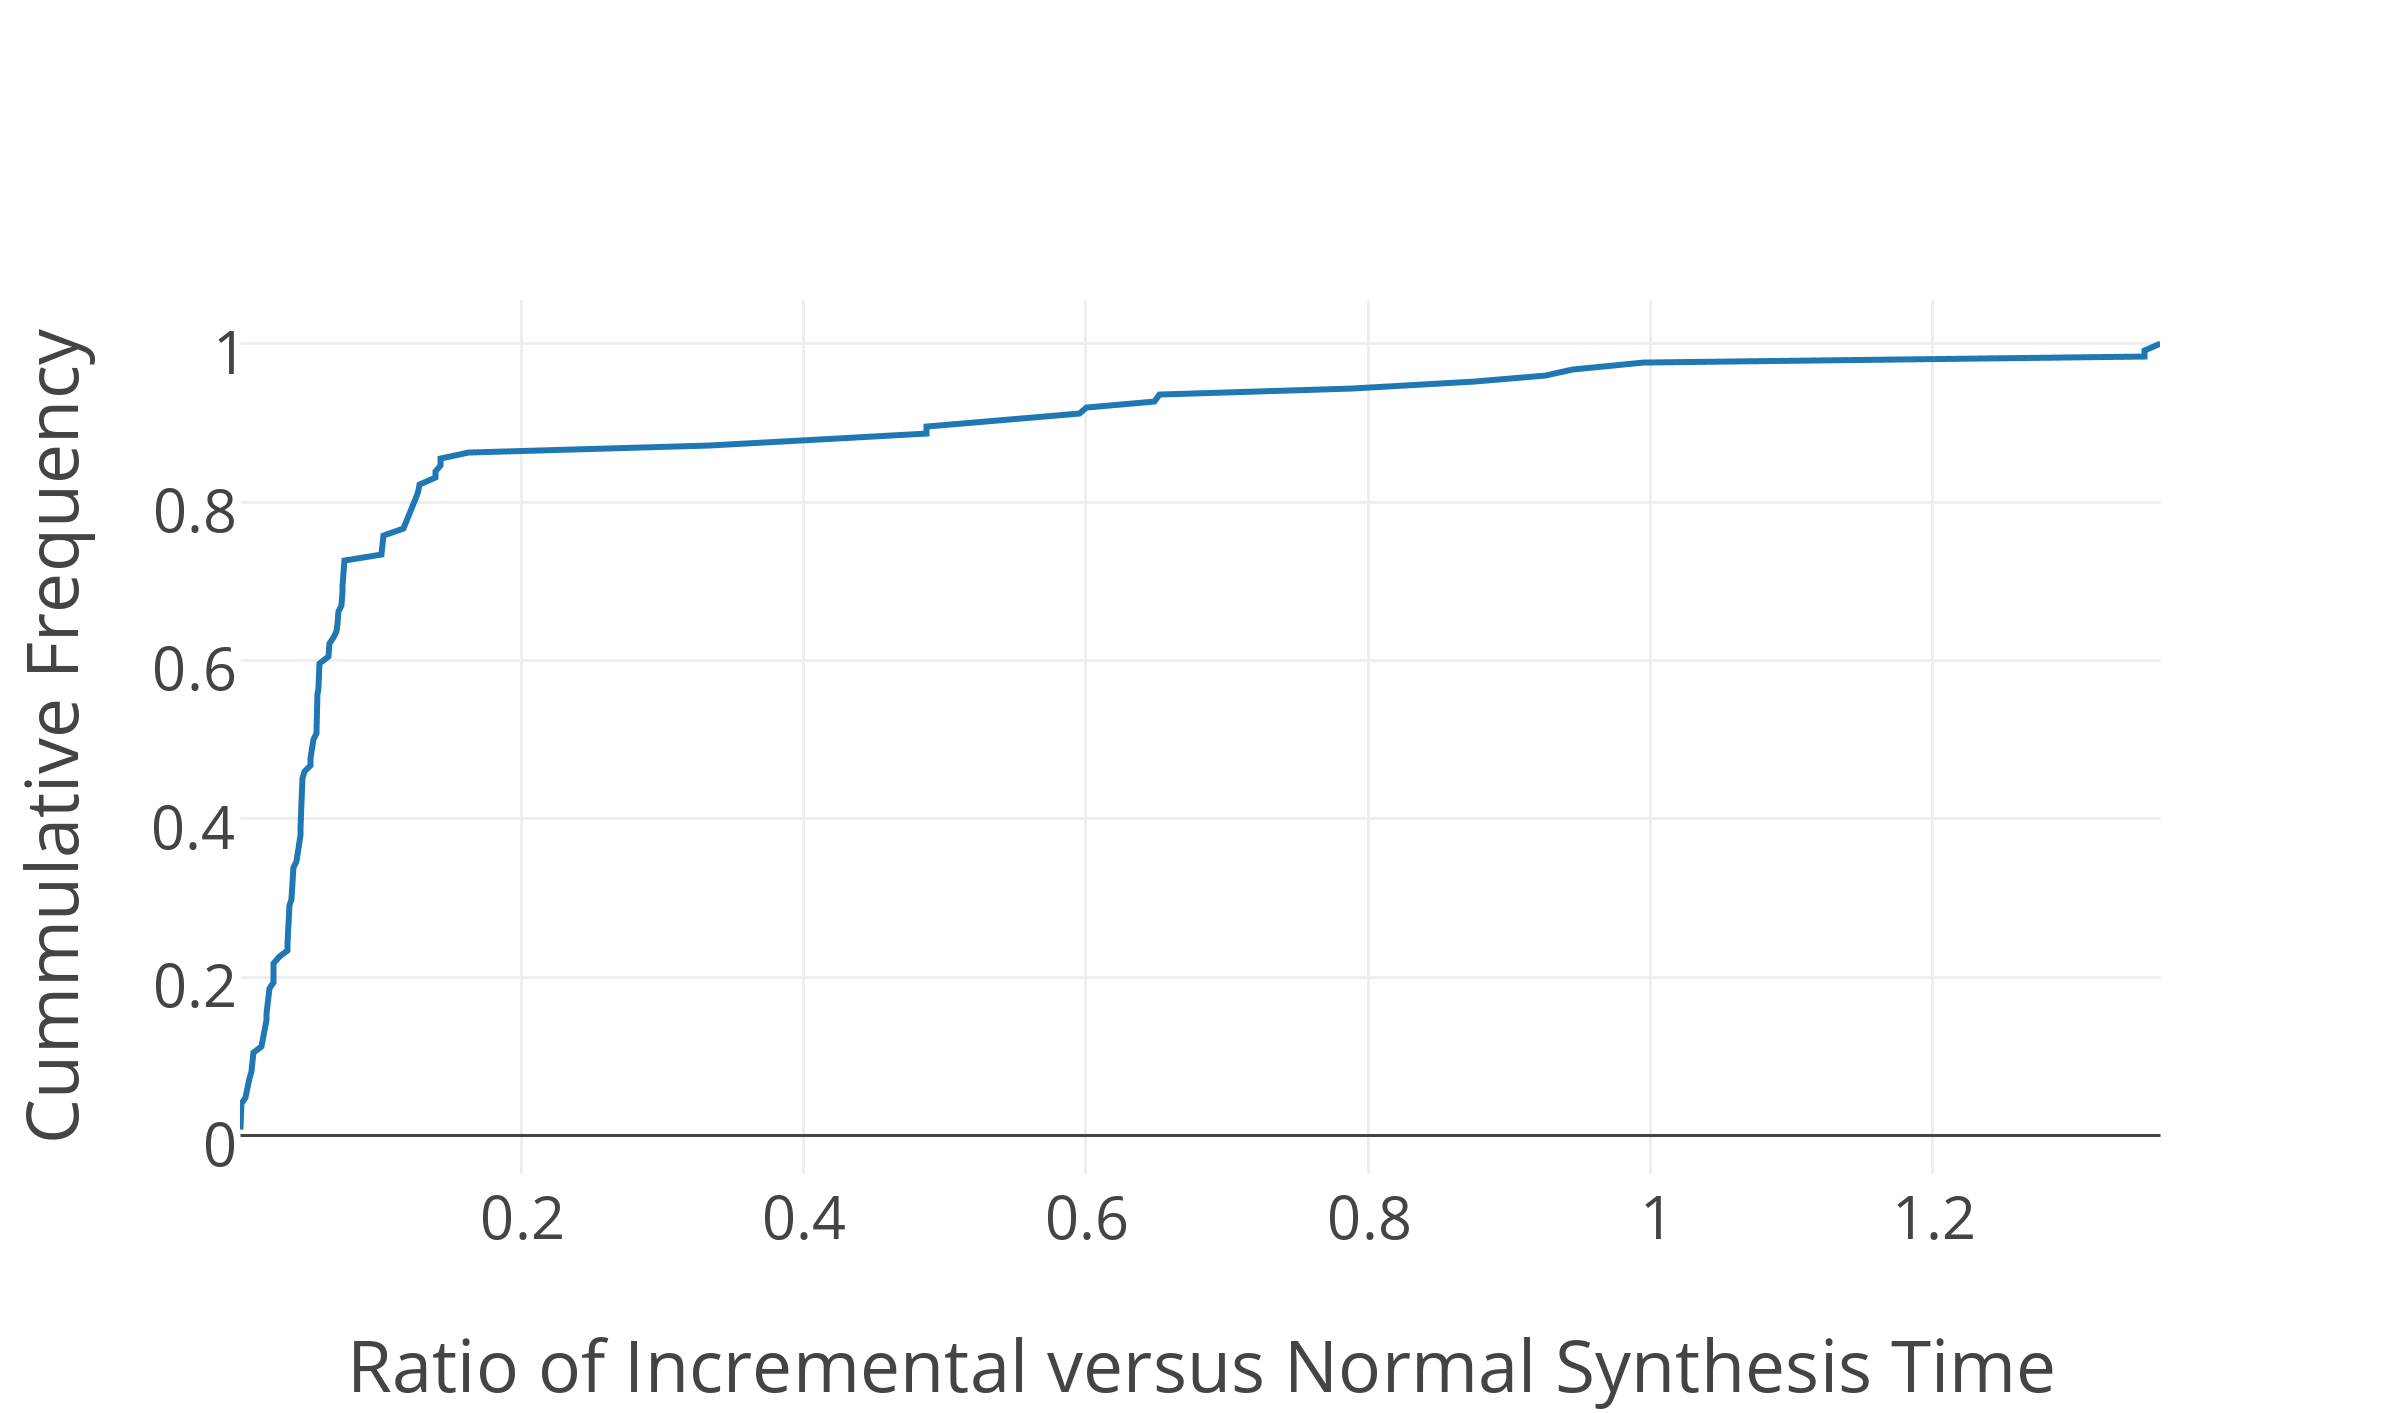
\includegraphics[width=0.5\columnwidth]{figures/incremental-cdf.eps}}
%	\caption{\label{fig:cdf}
%		Cumulative frequency distribution over 100 runs of isolation workloads for optimistic and incremental synthesis.}
%\end{figure}

%\begin{figure}
%	\centering
%	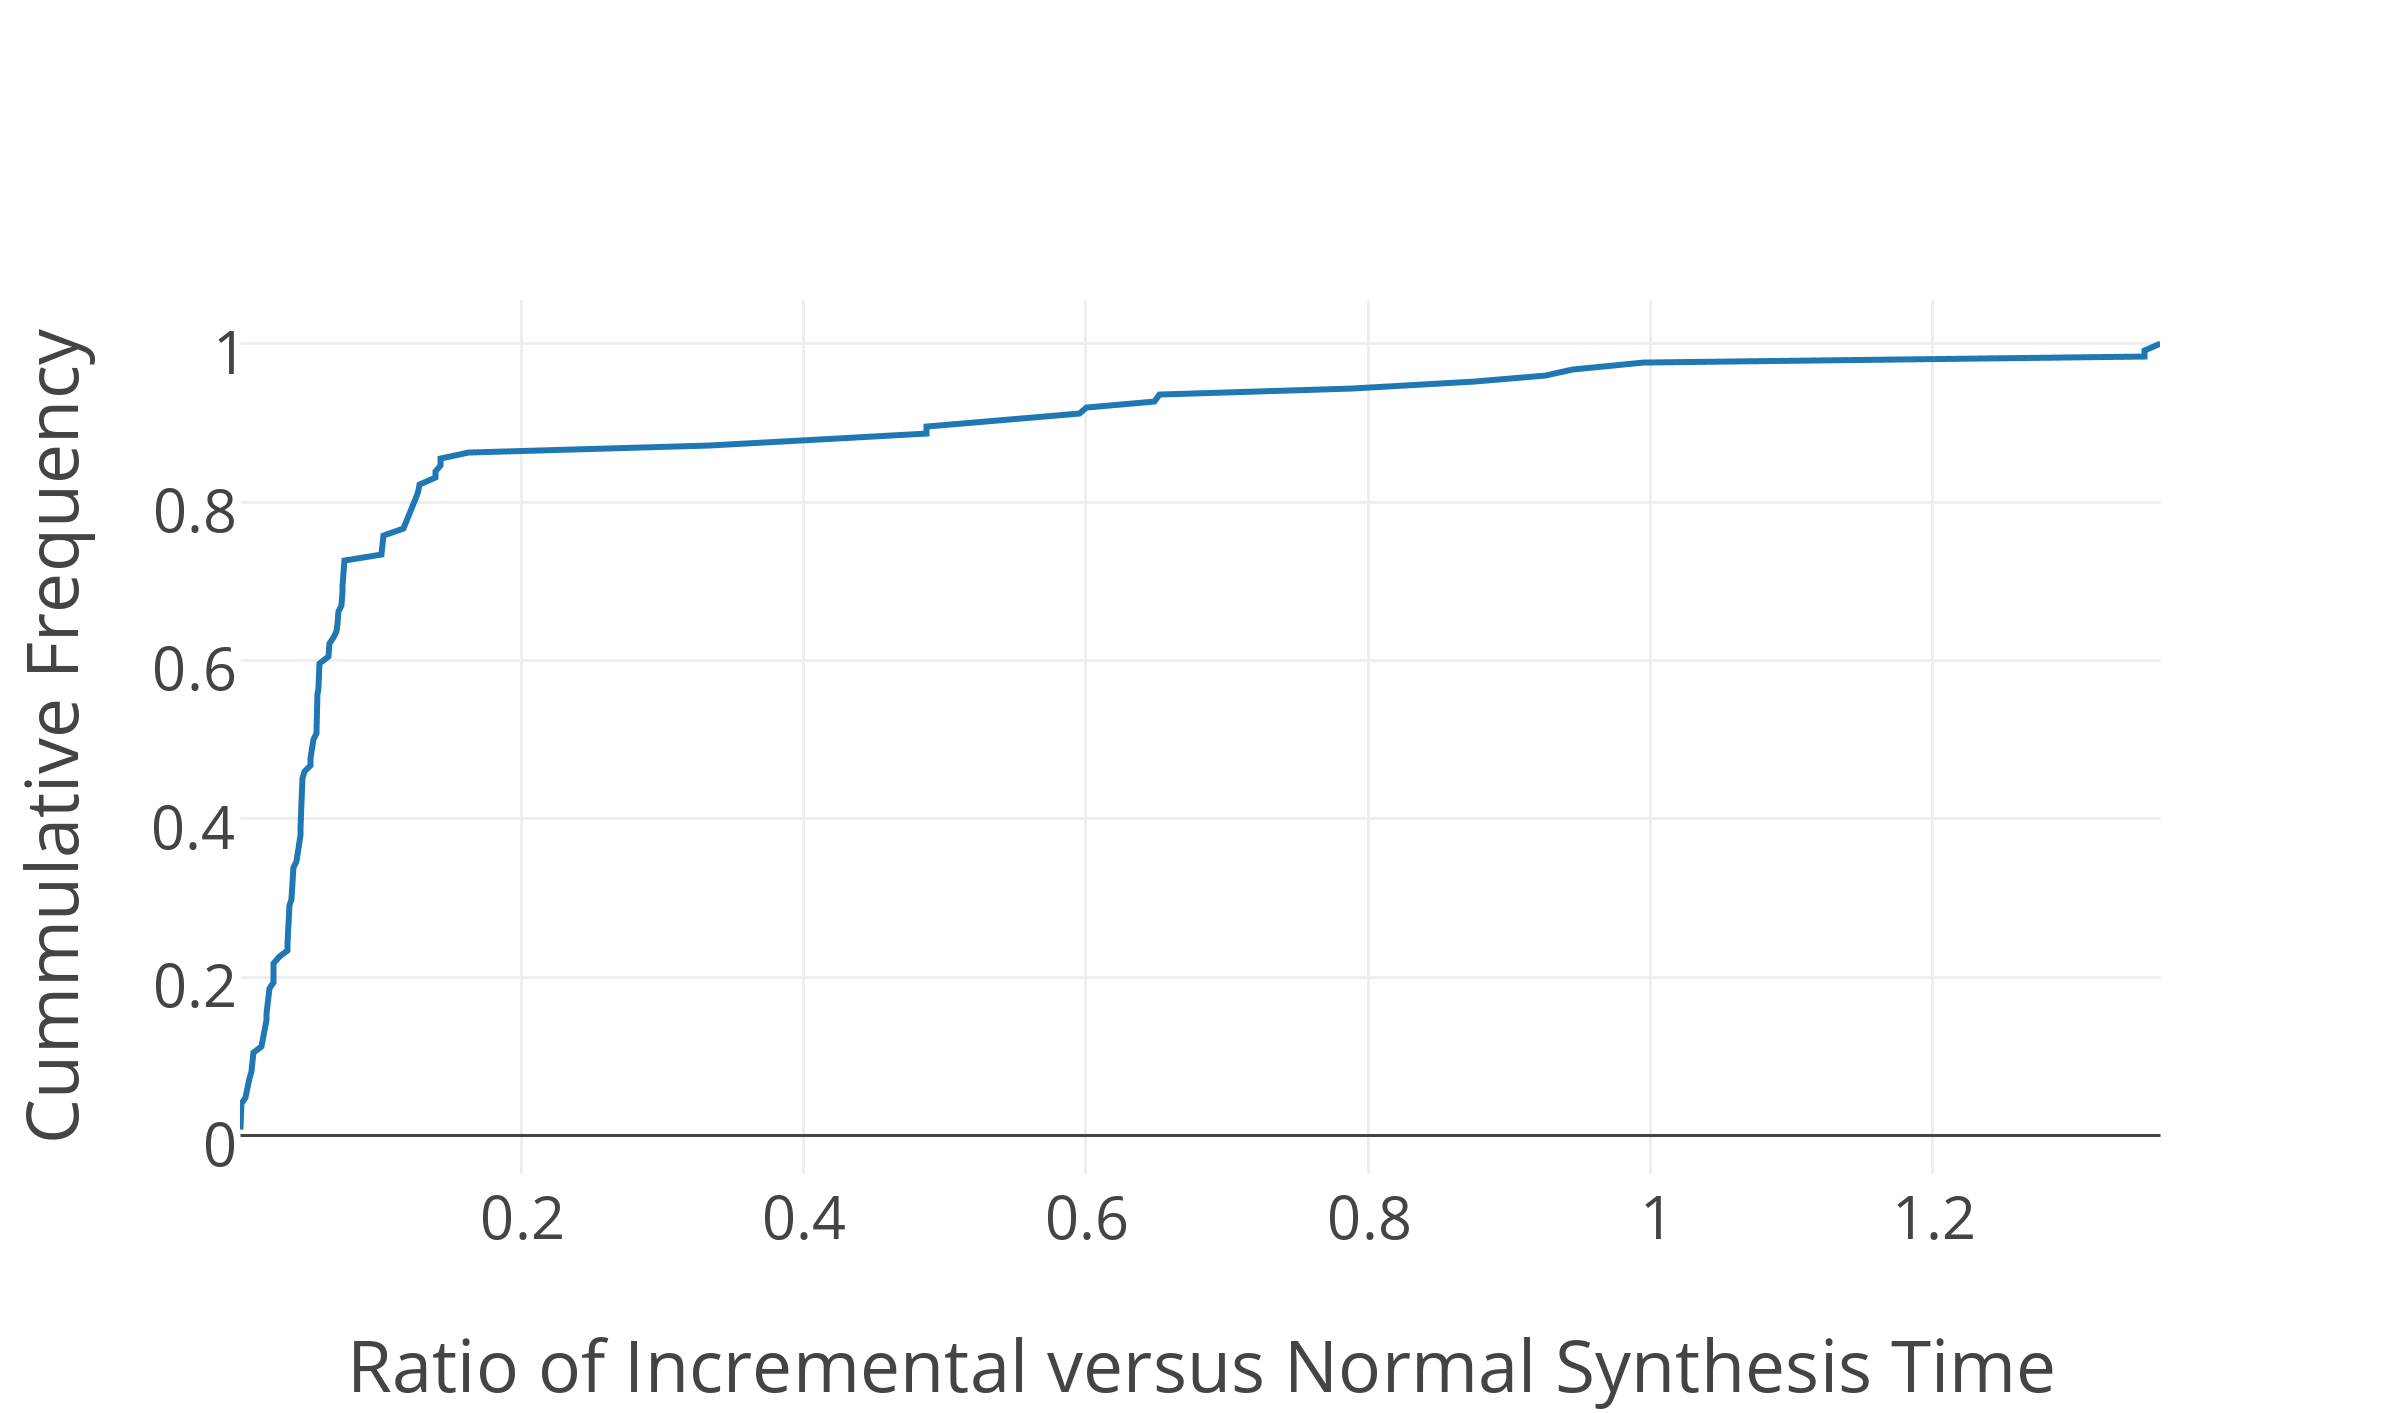
\includegraphics[width=0.75\columnwidth]{figures/incremental-cdf.eps}
%	\caption{CDF for ratio of incremental synthesis time over "one-shot" total synthesis time.}
%	\label{fig:incremental-cdf}
%\end{figure}


%\caption{Synthesis Time for varying number of reachability (with and without tactics) and waypoints policies for a 45 node fat-tree topology}


